\documentclass[12pt,a4paper,twoside]{report}
% -------------------------------------------------------------------- %
% Pacotes

\usepackage[utf8]{inputenc}
\usepackage[T1]{fontenc}
\usepackage[brazil]{babel}
\usepackage[fixlanguage]{babelbib}
\usepackage[pdftex]{graphicx}      % usamos arquivos pdf/png como figuras
\usepackage{setspace}              % espaçamento flexvel
\usepackage{indentfirst}           % indentação do primeiro parágrafo
\usepackage{makeidx}               % índice remissivo
\usepackage[nottoc]{tocbibind}     % acrescentamos a bibliografia/indice/conteudo no Table of Contents
\usepackage{courier}               % usa o Adobe Courier no lugar de Computer Modern Typewriter
\usepackage{type1cm}               % fontes realmente escaláveis
\usepackage{titletoc}
\usepackage{ucs}
\usepackage[font=small,format=plain,labelfont=bf,up,textfont=it,up]{caption}
\usepackage[usenames,svgnames,dvipsnames]{xcolor}
\usepackage[a4paper,top=2.54cm,bottom=2.0cm,left=2.0cm,right=2.54cm]{geometry} % margens
\usepackage{amsmath} 
\usepackage{float}

\usepackage[pdftex,plainpages=false,pdfpagelabels,pagebackref,colorlinks=true,citecolor=DarkGreen,
linkcolor=NavyBlue,urlcolor=DarkRed,filecolor=green,bookmarksopen=true]{hyperref} % links coloridos
\usepackage[all]{hypcap}                % soluciona o problema com o hyperref e capítulos
\usepackage[square,sort,nonamebreak,comma]{natbib}  % citação bibliográfica alpha
\fontsize{60}{62}\usefont{OT1}{cmr}{m}{n}{\selectfont}
\usepackage{upquote}                    % formata apóstrofes '
\usepackage{textcomp}

% Para formatar corretamente as URLs
\usepackage{url}
% -------------------------------------------------------------------- %
% Cabeçalhos similares ao TAOCP de Donald E. Knuth
\usepackage{fancyhdr}
\pagestyle{fancy}
\fancyhf{}
\renewcommand{\chaptermark}[1]{\markboth{\MakeUppercase{#1}}{}}
\renewcommand{\sectionmark}[1]{\markright{\MakeUppercase{#1}}{}}
\renewcommand{\headrulewidth}{0pt}

% -------------------------------------------------------------------- %
\graphicspath{{./imagens/}}        % caminho das figuras
\frenchspacing                     % arruma o espaço: id est (i.e.) e exempli gratia (e.g.)
\urlstyle{same}                    % URL com o mesmo estilo do texto e no mono-spaced
\makeindex                         % para o índice remissivo
\raggedbottom                      % para no permitir espaços extras no texto
\fontsize{60}{62}\usefont{OT1}{cmr}{m}{n}{\selectfont}
\cleardoublepage
\normalsize

% -------------------------------------------------------------------- %
% Cores para formatação de código
\usepackage{color}
\definecolor{vermelho}{rgb}{0.6,0,0} % para strings
\definecolor{verde}{rgb}{0.25,0.5,0.35} % para comentários
\definecolor{roxo}{rgb}{0.5,0,0.35} % para palavras-chaves
\definecolor{azul}{rgb}{0.25,0.35,0.75} % para strings
\definecolor{cinza-claro}{gray}{0.95}
% -------------------------------------------------------------------- %
% Opções de listagem usados para o código fonte
% Ref: http://en.wikibooks.org/wiki/LaTeX/Packages/Listings



\usepackage{listings}           % para formatar código-fonte (ex. em Java)


\lstset{ %
language=[Objective]Caml,  % seleciona a linguagem do código (aqui em lstlang0.sty
basicstyle=\footnotesize\ttfamily, % o tamanho da fonte usado no código
commentstyle=\color{verde}\bfseries,  % formatação de comentários
stringstyle=\color{azul},    % formatação de strings
upquote=true,
numbers=left,                   % onde colocar os números de linha
numberstyle=\tiny,  % o tamanho da fonte usada para a numeração das linhas
stepnumber=1,                   % o intervalo entre dois números de linhas. Se for 1, numera cada uma.
numbersep=5pt,                  % how far the line-numbers are from the code
showspaces=false,               % show spaces adding particular underscores
showstringspaces=false,         % underline spaces within strings
showtabs=false,                 % show tabs within strings adding particular underscores
keywordstyle=\color{roxo}\bfseries,
keywordstyle=[1]\color{roxo}\bfseries,
keywordstyle=[2]\color{verde}\bfseries,
%        keywordstyle=[3]\textbf,    %
%        keywordstyle=[4]\textbf,   \sqrt{\sqrt{}} %
frame=b,                   % adds a frame around the code
framerule=0.6pt,
tabsize=2,                      % sets default tabsize to 2 spaces
captionpos=t,                   % sets the caption-position to top
breaklines=true,                % sets automatic line breaking
breakatwhitespace=false,        % sets if automatic breaks should only happen at whitespace
escapeinside={\%*}{*)},         % if you want to add a comment within your code
backgroundcolor=\color[rgb]{1.0,1.0,1.0}, % choose the background color.
rulecolor=\color[rgb]{0.8,0.8,0.8},
extendedchars=true,
xleftmargin=10pt,
xrightmargin=10pt,
framexleftmargin=10pt,
framexrightmargin=10pt,
literate={â}{{\^{a}}}1  % para formatar corretamente os acentos do Português ao usar utf8
    {ê}{{\^{e}}}1
    {ô}{{\^{o}}}1  
    {Â}{{\^{A}}}1
    {Ê}{{\^{E}}}1
    {Ô}{{\^{O}}}1
    {á}{{\'{a}}}1
    {é}{{\'{e}}}1
    {í}{{\'{i}}}1
    {ó}{{\'{o}}}1
    {ú}{{\'{u}}}1
    {Á}{{\'{A}}}1
    {É}{{\'{E}}}1
    {Í}{{\'{I}}}1
    {Ó}{{\'{O}}}1
    {Ú}{{\'{U}}}1
    {à}{{\`{a}}}1
    {À}{{\`{A}}}1
    {ã}{{\~{a}}}1
    {õ}{{\~{o}}}1
    {Ã}{{\~{A}}}1
    {Õ}{{\~{O}}}1
    {ç}{{\c{c}}}1
    {Ç}{{\c{C}}}1
    {ü}{{\"u}}1
    {Ü}{{\"U}}1
}

\renewcommand{\lstlistingname}{Listagem}
\renewcommand{\lstlistlistingname}{Lista de Listagens}

% Definição de novos estilos
\lstdefinestyle{Bash}
    {language=bash,frame=single,numbers=none,basicstyle=\footnotesize\ttfamily,
     morekeywords={cp,mkdir,sudo,tar}}

% Definição de novos ambientes
\lstnewenvironment{terminal}
  {\lstset{style=Bash}}
  {}

\lstnewenvironment{ocaml}
  {\lstset{basicstyle=\scriptsize\ttfamily,
           frame=single,
           frameround=tttt,
           framerule=2pt,
           numbers=none,
           rulecolor=\color{Salmon}}}
  {}

\lstnewenvironment{xml}
   {\lstset{language=XML,frame=single,numbers=none}}
   {}

\lstnewenvironment{interprete}
  {\lstset{frame=single,
            frameround=tttt,
            numbers=none,
            basicstyle=\ttfamily,
            framerule=2pt,
            rulecolor=\color{CadetBlue}}}
  {}
% Formata o caption da listagem
% \DeclareCaptionFont{blue}{\color{blue}} 

% \captionsetup[lstlisting]{singlelinecheck=false, labelfont={blue}, textfont={blue}}
\usepackage{caption}
\DeclareCaptionFont{white}{\color{white}}
\DeclareCaptionFormat{listing}{\colorbox[cmyk]{0.43, 0.35, 0.35,0.01}{\parbox{\textwidth}{\hspace{15pt}#1#2#3}}}
\captionsetup[lstlisting]{format=listing,labelfont=white,textfont=white, singlelinecheck=false, margin=0pt, font={bf,footnotesize}}

\newcommand{\ListingsPath}{./codigos}
% Inclui o nome do arquivo como Caption 
\newcommand{\filelisting}[2][]{%
    \lstinputlisting[caption={\texttt{\detokenize{#2}}},#1]{\ListingsPath/#2}%
}

% ---------------------------------------------------------------------------- %

% ---------------------------------------------------------------------------- %

\title{Análise de Algoritmos - Ordenação}
\date{}
\author{Gustavo de Souza Silva \\ Guilherme de Souza Silva \\ Arthur Xavier \\ Schumaiquer Souto \\
\vspace{1cm} \\
Faculdade de Computação \\
Universidade Federal de Uberlândia
}
\date{\today}

%\includeonly{cap-clojure,magical,short}
\begin{document}
  \maketitle
% -------------------------------------------------------------------- %
% Listas de figuras, tabelas e códigos criadas automaticamente
\listoffigures            
\listoftables            
\lstlistoflistings
% -------------------------------------------------------------------- %

% -------------------------------------------------------------------- %
% Sumário
\tableofcontents    

% Capítulos do trabalho

% cabeçalho para as páginas de todos os capítulos
\fancyhead[RE,LO]{\thesection}

%\singlespacing              % espaçamento simples
\setlength{\parskip}{0.15in} % espaçamento entre paragráfos

\chapter{Introdução}
Este relatório tem como objetivo fazer a análise de diversos algoritmos já conhecidos de ordenação. O intuito deste trabalho é comprovar que as provas matemáticas realmente acontecem em um ambiente real de execução.

\section{Codificação}
O arquivo vetor.c mantém todas as funções a respeito do vetor, como geração, preenchimento, etc.
\lstinputlisting[label={arq:vetor.c}, language=C, caption={Arquivo referente ao vetor}]{../vetor.c}

Este arquivo serve para gerar os vetores e salva-los em arquivos.
\lstinputlisting[label={arq:gera_vets.c}, language=C, caption={Geração dos vetores}]{../gera_vets.c}

Este arquivo contém os algoritmos de ordenação pedidos.
\lstinputlisting[label={arq:ordena.c}, language=C, caption={Métodos de ordenação}]{../ordena.c}

O arquivo ensaios.c serve para automatizar e calcular os tempos de cada método de ordenação.
\lstinputlisting[label={arq:ensaios.c}, language=C, caption={Automatização dos experimentos}]{../ensaios.c}

\subsection{Comandos}
Os seguintes passos devem ser seguidos para criação dos vetores que serão utilizados no experimento:\\
1 - Compilar o arquivo vetor.c;
\begin{terminal}
    > gcc -O3 -c vetor.c
\end{terminal}
2 - Compilar o programa que gera os vetores e os coloca no diretório determinado;
\begin{terminal}
    > gcc -O3 vetor.o gera_vets.c -o gera_vets.exe
\end{terminal}
3 - Para usá-lo digite
\begin{terminal}
    > ./gera_vets.exe
\end{terminal}

Os passos a seguir são para execução do experimento\\
1 - Verifique a existência do diretório contendo os vetores, e então digite o seguinte comando:
\begin{terminal}
    > gcc -O3 -c ordena.c
\end{terminal}
2 - Agora é necessário compilar o arquivo de ensaio e tudo que será utilizado
\begin{terminal}
    > gcc -O3 vetor.o ordena.o ensaios.c -o ensaios.exe -lm
\end{terminal}
3 - Para executar digite:
\begin{terminal}
    > ./ensaios.exe
\end{terminal}

\section{Máquina de teste}
Todos os testes foram realizados na mesma máquina com as seguintes configurações, e usando apenas um núcleo:\\
AMD FX-8350 4.0GHZ\\
16GB Memória DDR3-1600\\
HDD 2TB 7200RPM\\
Placa de video Nvidia GTX1050Ti\\
Sistema Operacional: Ubuntu 16.04\\

\chapter{Grafo}

balbalbalbal

\section{Busca Largura}

É um algoritmo de busca em grafos utilizado para realizar uma busca ou travessia num grafo e estrutura de dados do tipo árvore. Você começa pelo vértice raiz e explora todos os vértices vizinhos. Então, para cada um desses vértices mais próximos, exploramos os seus vértices vizinhos inexplorados e assim por diante, até que ele encontre o alvo da busca.

\section{Busca Largura - Grafo Esparso}
Tabela gerada utilizando Busca em largura com grafo esparso de tamanho n, sendo = $(2^k)$, k = 4...14.
\begin{table}[H]
\centering
\caption{Busca Largura com grafo Esparso}
\begin{tabular}{|l|l|}
\hline
\multicolumn{1}{|c|}{\textbf{Número de Elementos}} & \multicolumn{1}{c|}{\textbf{Tempo de execução em nanosegundos}} \\ \hline
128 & 7943 \\ \hline
256 & 7472 \\ \hline
512 & 15414 \\ \hline
1024 & 32102 \\ \hline
\end{tabular}
\end{table}

\subsection{Gráfico Busca Largura - Grafo Esparso}
\begin{figure}[H]
    \centering
    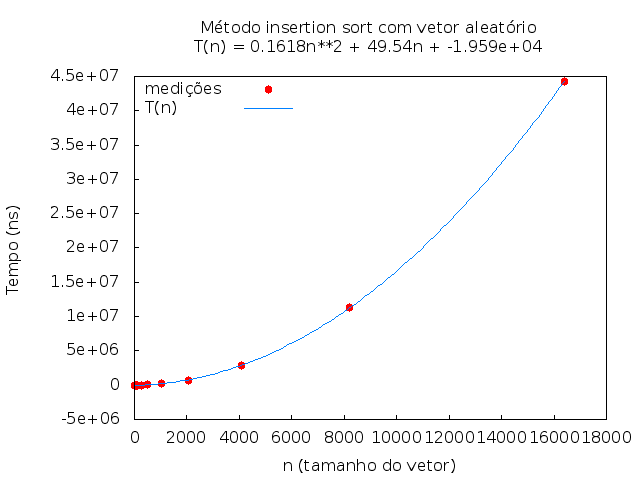
\includegraphics[width=0.7\linewidth]{graficos/Insertion/vIntAleatorio/vIntAleatorio.png}
  \caption{Busca Largura - Grafo Esparso}
\end{figure}

\section{Busca Largura - Grafo Denso}
Tabela gerada utilizando Busca em Largura num grafo Denso com n, sendo = $(2^k)$, k = 4...14.

\begin{table}[H]
\centering
\caption{Busca em Largura Grafo Denso}
\label{my-label}
\begin{tabular}{|l|l|}
\hline
\multicolumn{1}{|c|}{\textbf{Número de Elementos}} & \multicolumn{1}{c|}{\textbf{Tempo de execução em nanosegundos}} \\ \hline
128 & 67546 \\ \hline
256 & 318565 \\ \hline
512 & 1216634 \\ \hline
1024 & 4527417 \\ \hline
\end{tabular}
\end{table}

\subsection{Busca em Largura - Grafo Denso}
\begin{figure}[H]
    \centering
    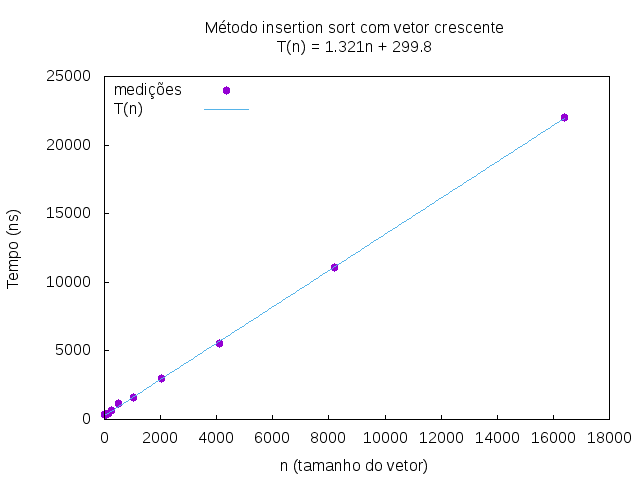
\includegraphics[width=0.7\linewidth]{graficos/Insertion/vIntCrescente/vIntCrescente.png}
  \caption{Busca em Largura - Grafo Denso}
\end{figure}

\section{Busca Profundidade}
É um algoritmo usado para realizar uma busca ou travessia numa árvore, estrutura de árvore ou grafo. O algoritmo começa num nó raiz (selecionando algum nó como sendo o raiz, no caso de um grafo) e explora tanto quanto possível cada um dos seus ramos, antes de retroceder(backtracking).

\section{Busca Profundidade - Grafo Esparso}
Tabela gerada utilizando Busca Profundidade com um Grafo Esparso, sendo n = $(2^k)$, de k = 4..14.
\begin{table}[H]
\centering
\caption{Busca Profundidade com Grafo Esparso}
\label{my-label}
\begin{tabular}{|l|l|}
\hline
\multicolumn{1}{|c|}{\textbf{Número de Elementos}} & \multicolumn{1}{c|}{\textbf{Tempo de execução em nanosegundos}} \\ \hline
128 & 6619 \\ \hline
256 & 7975 \\ \hline
512 & 21265 \\ \hline
1024 & 36223 \\ \hline
\end{tabular}
\end{table}

\subsection{Busca Profundidade - Grafo Esparso}
\begin{figure}[H]
    \centering
    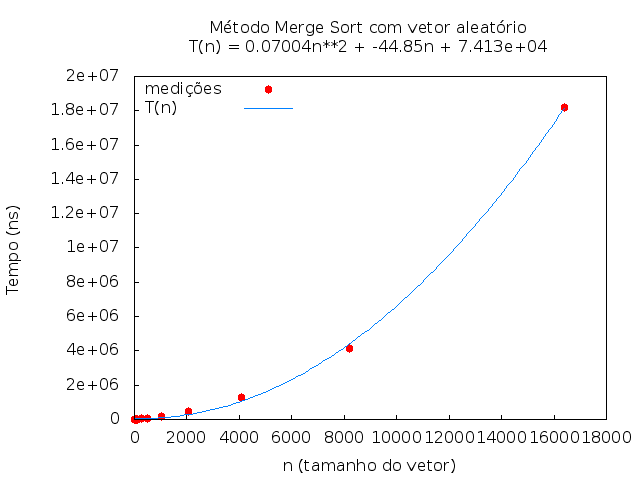
\includegraphics[width=0.7\linewidth]{graficos/MergeSort/vIntAleatorio/vIntAleatorio.png}
  \caption{Busca Profundidade - Grafo Esparso}
\end{figure}

\section{Busca Profundidade - Grafo Denso}
Tabela gerada utilizando Busca em Profundidade com um Grafo Denso, sendo n = $(2^k)$, de k = 4..14.
\begin{table}[H]
\centering
\caption{Busca Profundidade em um Grafo Denso}
\label{my-label}
\begin{tabular}{|l|l|}
\hline
\multicolumn{1}{|c|}{\textbf{Número de Elementos}} & \multicolumn{1}{c|}{\textbf{Tempo de execução em nanosegundos}} \\ \hline
128 & 72161 \\ \hline
256 & 330916 \\ \hline
512 & 1380078 \\ \hline
1024 & 4735134 \\ \hline
\end{tabular}
\end{table}

\subsection{Busca Profundidade - Grafo Denso}
\begin{figure}[H]
    \centering
    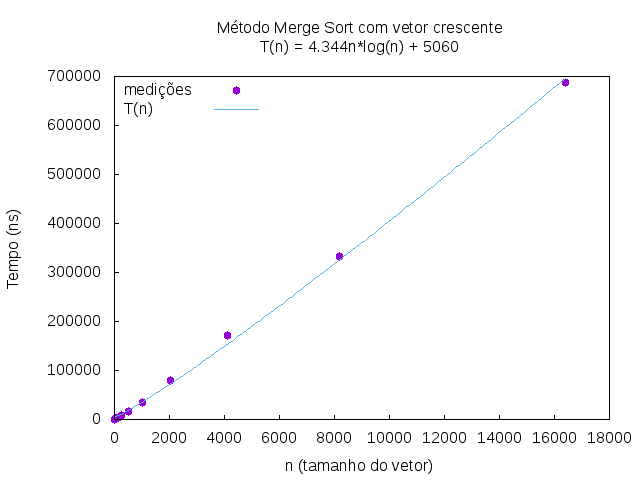
\includegraphics[width=0.7\linewidth]{graficos/MergeSort/vIntCrescente/vIntCrescente.png}
  \caption{Busca Profundidade - Grafo Denso}
\end{figure}

\section{Ordenação Topologica}

blabalblalbalbalb

\section{Ordenação Topologica - Grafo Esparso}
Tabela gerada utilizando Ordenação Topologica com um Grafo Esparso, sendo n = $(2^k)$, de k = 4..14.
\begin{table}[H]
\centering
\caption{Ordenação Topologica com Grafo Esparso}
\label{my-label}
\begin{tabular}{|l|l|}
\hline
\multicolumn{1}{|c|}{\textbf{Número de Elementos}} & \multicolumn{1}{c|}{\textbf{Tempo de execução em nanosegundos}} \\ \hline
128 & 13549 \\ \hline
256 & 15347 \\ \hline
512 & 30745 \\ \hline
1024 & 57293 \\ \hline
\end{tabular}
\end{table}

\subsection{Ordenação Topologica - Grafo Esparso}
\begin{figure}[H]
    \centering
    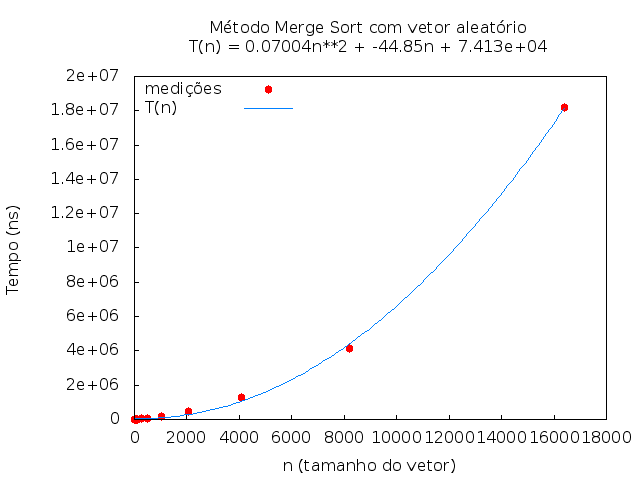
\includegraphics[width=0.7\linewidth]{graficos/MergeSort/vIntAleatorio/vIntAleatorio.png}
  \caption{Ordenação Topologica - Grafo Esparso}
\end{figure}

\section{Ordenação Topologica - Grafo Denso}
Tabela gerada utilizando Ordenação Topologica com um Grafo Denso, sendo n = $(2^k)$, de k = 4..14.
\begin{table}[H]
\centering
\caption{Ordenação Topologica com Grafo Denso}
\label{my-label}
\begin{tabular}{|l|l|}
\hline
\multicolumn{1}{|c|}{\textbf{Número de Elementos}} & \multicolumn{1}{c|}{\textbf{Tempo de execução em nanosegundos}} \\ \hline
128 & 93864 \\ \hline
256 & 349061 \\ \hline
512 & 1344655 \\ \hline
1024 & 4865168 \\ \hline
\end{tabular}
\end{table}

\subsection{Ordenação Topologica - Grafo Denso}
\begin{figure}[H]
    \centering
    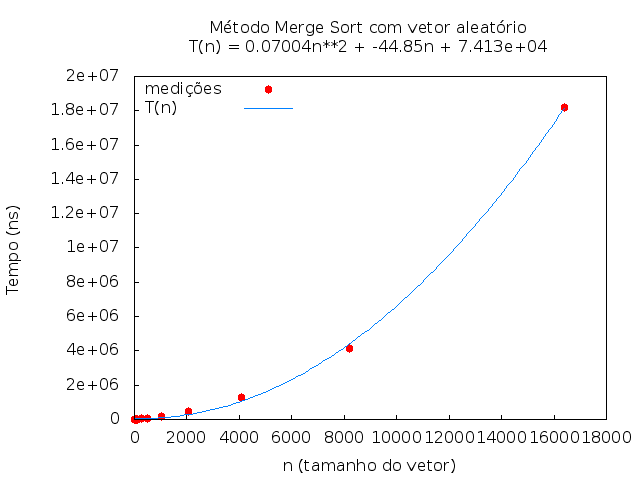
\includegraphics[width=0.7\linewidth]{graficos/MergeSort/vIntAleatorio/vIntAleatorio.png}
  \caption{Ordenação Topologica - Grafo Denso}
\end{figure}

\chapter{Guloso}

 blablabla

\section{Huffman}

blabalbal Vetor de string aleatorias com frequencias aleatorias
Tempo (Onlgn)

\subsection{Vetor aleatorio}
Tabela gerada utilizando Huffman com vetor de string aleatorias com frequencias em tempo O(nlogn) de tamanho n, sendo n = $(2^k)$, de k = 4..14 e inseridos aleatóriamente.
\begin{table}[H]
\centering
\caption{Huffman com vetor aleatório}
\label{my-label}
\begin{tabular}{|l|l|}
\hline
\multicolumn{1}{|c|}{\textbf{Número de Elementos}} & \multicolumn{1}{c|}{\textbf{Tempo de execução em nanosegundos}} \\ \hline
16 & 4599 \\ \hline
32 & 8150 \\ \hline
64 & 22736 \\ \hline
128 & 42886 \\ \hline
256 & 95255 \\ \hline
512 & 170503 \\ \hline
1024 & 438873 \\ \hline
2048 & 1031620 \\ \hline
4096 & 2592036 \\ \hline
8192 & 5381493 \\ \hline
16384 & 10506005 \\ \hline

\end{tabular}
\end{table}

\begin{figure}[H]
    \centering
    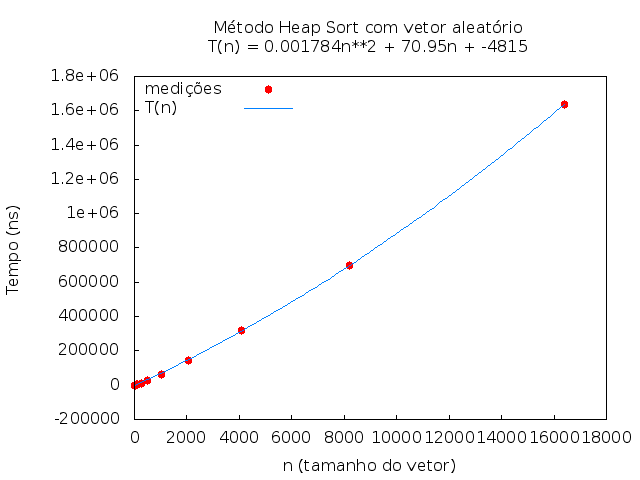
\includegraphics[width=0.7\linewidth]{graficos/HeapSort/vIntAleatorio/vIntAleatorio.png}
  \caption{Huffman - Vetor Aleatório}
\end{figure}

\section{Seleção de Atividade Interativo}

blabalbal 

\subsection{Vetor crescente}
Tabela gerada utilizando Seleção de Atividade Interativo com vetor de tamanho n, sendo n = $(2^k)$, de k = 4..14 e inseridos crescente.
\begin{table}[H]
\centering
\caption{Seleção de Atividade Interativo com vetor crescente}
\label{my-label}
\begin{tabular}{|l|l|}
\hline
\multicolumn{1}{|c|}{\textbf{Número de Elementos}} & \multicolumn{1}{c|}{\textbf{Tempo de execução em nanosegundos}} \\ \hline
16 & 615 \\ \hline
32 & 680 \\ \hline
64 & 769 \\ \hline
128 & 802 \\ \hline
256 & 764 \\ \hline
512 & 836 \\ \hline
1024 & 1058 \\ \hline
2048 & 1294 \\ \hline
4096 & 1685 \\ \hline
8192 & 2594 \\ \hline
16384 & 4578 \\ \hline

\end{tabular}
\end{table}

\begin{figure}[H]
    \centering
    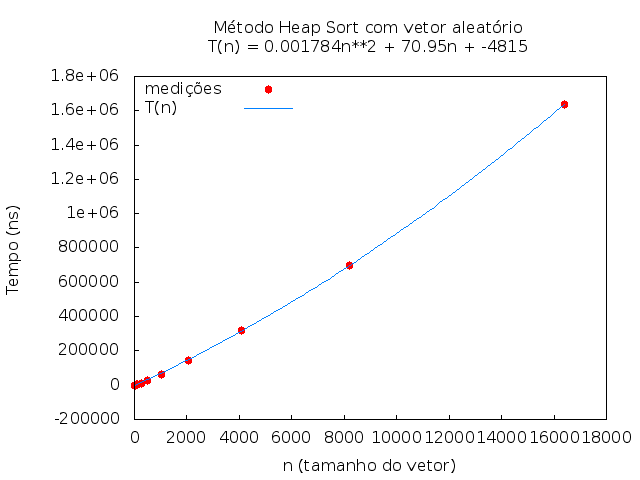
\includegraphics[width=0.7\linewidth]{graficos/HeapSort/vIntAleatorio/vIntAleatorio.png}
  \caption{Seleção de Atividade Interativo - Vetor crescente}
\end{figure}


\section{Seleção de Atividade Bottom Up}

blabalbal 

\subsection{Vetor crescente}
Tabela gerada utilizando Seleção de Atividade Bottom Up com vetor de tamanho n, sendo n = $(2^k)$, de k = 4..14 e inseridos crescente.
\begin{table}[H]
\centering
\caption{Seleção de Atividade Bottom Up com vetor crescente}
\label{my-label}
\begin{tabular}{|l|l|}
\hline
\multicolumn{1}{|c|}{\textbf{Número de Elementos}} & \multicolumn{1}{c|}{\textbf{Tempo de execução em nanosegundos}} \\ \hline
16 & 615 \\ \hline
32 & 680 \\ \hline
64 & 769 \\ \hline
128 & 802 \\ \hline
256 & 764 \\ \hline
512 & 836 \\ \hline
1024 & 1058 \\ \hline
2048 & 1294 \\ \hline
4096 & 1685 \\ \hline
8192 & 2594 \\ \hline
16384 & 4578 \\ \hline

\end{tabular}
\end{table}

\begin{figure}[H]
    \centering
    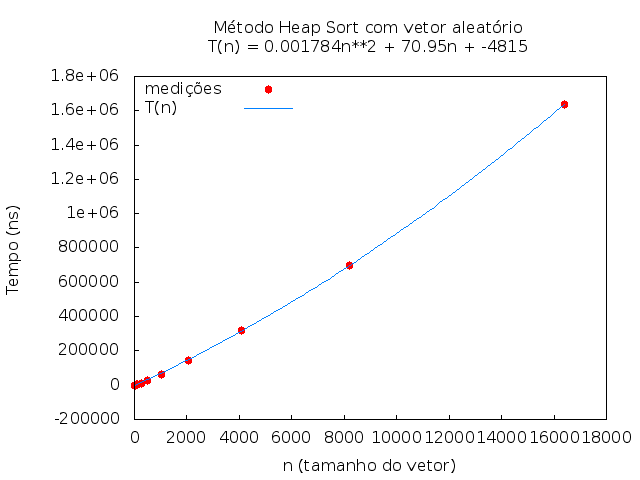
\includegraphics[width=0.7\linewidth]{graficos/HeapSort/vIntAleatorio/vIntAleatorio.png}
  \caption{Seleção de Atividade Bottom Up - Vetor crescente}
\end{figure}


\chapter{Programação Dinâmica}

Programação dinamica blablabla
\section{Corte Haste}
Falar sobre corte de hastes comum
+dados
falar o que deu errado.
Será resolvido utilizando programação dinâmica.

\section{Corte Haste Bottom Up}

falar um pouco sobre bottomup (n muito).

\subsection{Vetor aleatorio}
Tabela gerada utilizando Corte Haste Bottom Up com vetores de tamanho n, sendo n = $(2^k)$, de k = 4..14 e inseridos aleatóriamente.
\begin{table}[H]
\centering
\caption{Corte Haste Bottom Up com vetor aleatório}
\label{my-label}
\begin{tabular}{|l|l|}
\hline
\multicolumn{1}{|c|}{\textbf{Número de Elementos}} & \multicolumn{1}{c|}{\textbf{Tempo de execução em nanosegundos}} \\ \hline
16 & 599 \\ \hline
32 & 913 \\ \hline
64 & 1798 \\ \hline
128 & 4618 \\ \hline
256 & 14530 \\ \hline
512 & 51214 \\ \hline
1024 & 193794 \\ \hline
2048 & 761470 \\ \hline
4096 & 2965012 \\ \hline
8192 & 12774326 \\ \hline
16384 & 48066532 \\ \hline
\end{tabular}
\end{table}

\begin{figure}[H]
    \centering
    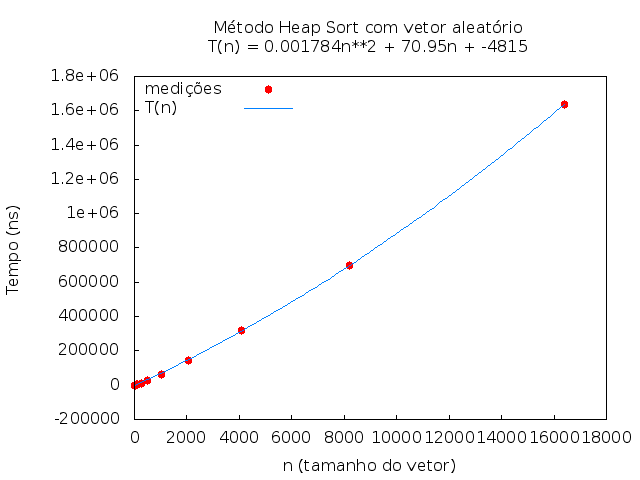
\includegraphics[width=0.7\linewidth]{graficos/HeapSort/vIntAleatorio/vIntAleatorio.png}
  \caption{Corte Haste Bottom Up - Vetor Aleatório}
\end{figure}


\subsection{Vetor Crescente}
Tabela gerada utilizando Corte Haste Bottom Up com vetores de tamanho n, sendo n = $(2^k)$, de k = 4..14 e inseridos de forma crescente.
\begin{table}[H]
\centering
\caption{Corte Haste Bottom Up com Vetor Crescente}
\label{my-label}
\begin{tabular}{|l|l|}
\hline
\multicolumn{1}{|c|}{\textbf{Número de Elementos}} & \multicolumn{1}{c|}{\textbf{Tempo de execução em nanosegundos}} \\ \hline
16 & 599 \\ \hline
32 & 913 \\ \hline
64 & 1798 \\ \hline
128 & 4618 \\ \hline
256 & 14530 \\ \hline
512 & 51214 \\ \hline
1024 & 193794 \\ \hline
2048 & 761470 \\ \hline
4096 & 2965012 \\ \hline
8192 & 12774326 \\ \hline
16384 & 48066532 \\ \hline
\end{tabular}
\end{table}

\begin{figure}[H]
    \centering
    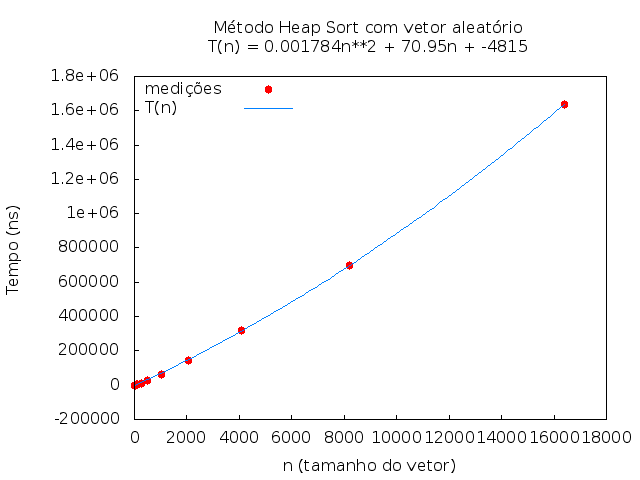
\includegraphics[width=0.7\linewidth]{graficos/HeapSort/vIntAleatorio/vIntAleatorio.png}
  \caption{Corte Haste Bottom Up - Vetor Crescente}
\end{figure}




\subsection{Vetor Crescente P10}
Tabela gerada utilizando Corte Haste Bottom Up com vetores de tamanho n, sendo n = $(2^k)$, de k = 4..14 e inseridos de forma crescente P10.
\begin{table}[H]
\centering
\caption{Corte Haste Bottom Up com Vetor Crescente P10}
\label{my-label}
\begin{tabular}{|l|l|}
\hline
\multicolumn{1}{|c|}{\textbf{Número de Elementos}} & \multicolumn{1}{c|}{\textbf{Tempo de execução em nanosegundos}} \\ \hline
16 & 599 \\ \hline
32 & 913 \\ \hline
64 & 1798 \\ \hline
128 & 4618 \\ \hline
256 & 14530 \\ \hline
512 & 51214 \\ \hline
1024 & 193794 \\ \hline
2048 & 761470 \\ \hline
4096 & 2965012 \\ \hline
8192 & 12774326 \\ \hline
16384 & 48066532 \\ \hline
\end{tabular}
\end{table}

\begin{figure}[H]
    \centering
    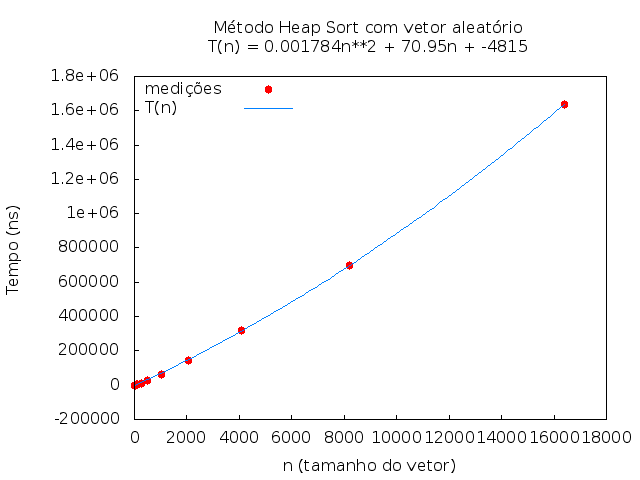
\includegraphics[width=0.7\linewidth]{graficos/HeapSort/vIntAleatorio/vIntAleatorio.png}
  \caption{Corte Haste Bottom Up - Vetor Crescente P10}
\end{figure}





\subsection{Vetor Crescente P20}
Tabela gerada utilizando Corte Haste Bottom Up com vetores de tamanho n, sendo n = $(2^k)$, de k = 4..14 e inseridos de forma crescente P20.
\begin{table}[H]
\centering
\caption{Corte Haste Bottom Up com Vetor Crescente P20}
\label{my-label}
\begin{tabular}{|l|l|}
\hline
\multicolumn{1}{|c|}{\textbf{Número de Elementos}} & \multicolumn{1}{c|}{\textbf{Tempo de execução em nanosegundos}} \\ \hline
16 & 599 \\ \hline
32 & 913 \\ \hline
64 & 1798 \\ \hline
128 & 4618 \\ \hline
256 & 14530 \\ \hline
512 & 51214 \\ \hline
1024 & 193794 \\ \hline
2048 & 761470 \\ \hline
4096 & 2965012 \\ \hline
8192 & 12774326 \\ \hline
16384 & 48066532 \\ \hline
\end{tabular}
\end{table}

\begin{figure}[H]
    \centering
    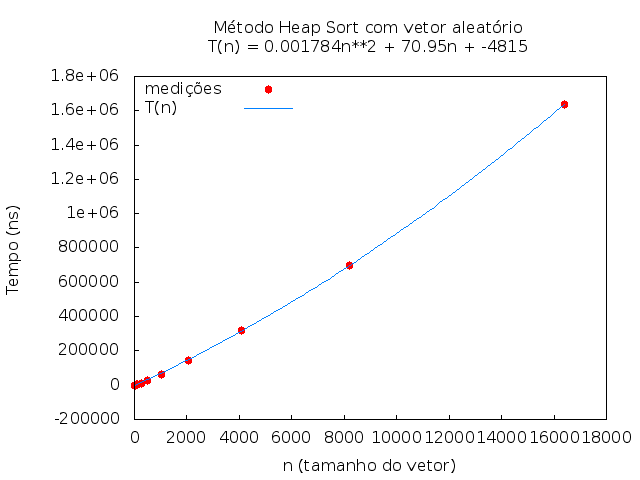
\includegraphics[width=0.7\linewidth]{graficos/HeapSort/vIntAleatorio/vIntAleatorio.png}
  \caption{Corte Haste Bottom Up - Vetor Crescente P20}
\end{figure}




\subsection{Vetor Crescente P30}
Tabela gerada utilizando Corte Haste Bottom Up com vetores de tamanho n, sendo n = $(2^k)$, de k = 4..14 e inseridos de forma crescente P30.
\begin{table}[H]
\centering
\caption{Corte Haste Bottom Up com Vetor Crescente P30}
\label{my-label}
\begin{tabular}{|l|l|}
\hline
\multicolumn{1}{|c|}{\textbf{Número de Elementos}} & \multicolumn{1}{c|}{\textbf{Tempo de execução em nanosegundos}} \\ \hline
16 & 599 \\ \hline
32 & 913 \\ \hline
64 & 1798 \\ \hline
128 & 4618 \\ \hline
256 & 14530 \\ \hline
512 & 51214 \\ \hline
1024 & 193794 \\ \hline
2048 & 761470 \\ \hline
4096 & 2965012 \\ \hline
8192 & 12774326 \\ \hline
16384 & 48066532 \\ \hline
\end{tabular}
\end{table}

\begin{figure}[H]
    \centering
    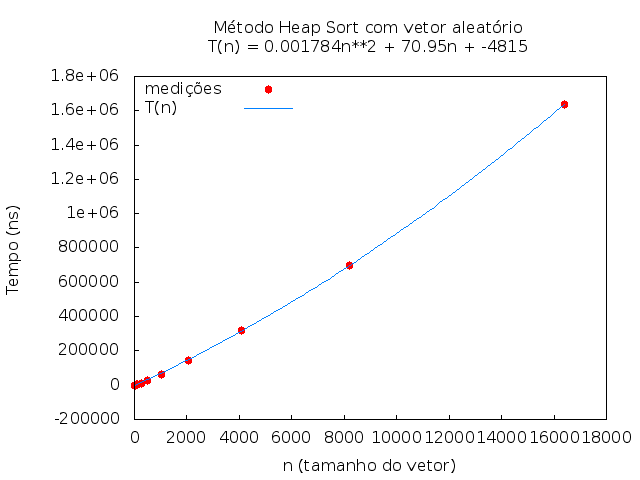
\includegraphics[width=0.7\linewidth]{graficos/HeapSort/vIntAleatorio/vIntAleatorio.png}
  \caption{Corte Haste Bottom Up - Vetor Crescente P30}
\end{figure}




\subsection{Vetor Crescente P40}
Tabela gerada utilizando Corte Haste Bottom Up com vetores de tamanho n, sendo n = $(2^k)$, de k = 4..14 e inseridos de forma crescente P40.
\begin{table}[H]
\centering
\caption{Corte Haste Bottom Up com Vetor Crescente P40}
\label{my-label}
\begin{tabular}{|l|l|}
\hline
\multicolumn{1}{|c|}{\textbf{Número de Elementos}} & \multicolumn{1}{c|}{\textbf{Tempo de execução em nanosegundos}} \\ \hline
16 & 599 \\ \hline
32 & 913 \\ \hline
64 & 1798 \\ \hline
128 & 4618 \\ \hline
256 & 14530 \\ \hline
512 & 51214 \\ \hline
1024 & 193794 \\ \hline
2048 & 761470 \\ \hline
4096 & 2965012 \\ \hline
8192 & 12774326 \\ \hline
16384 & 48066532 \\ \hline
\end{tabular}
\end{table}

\begin{figure}[H]
    \centering
    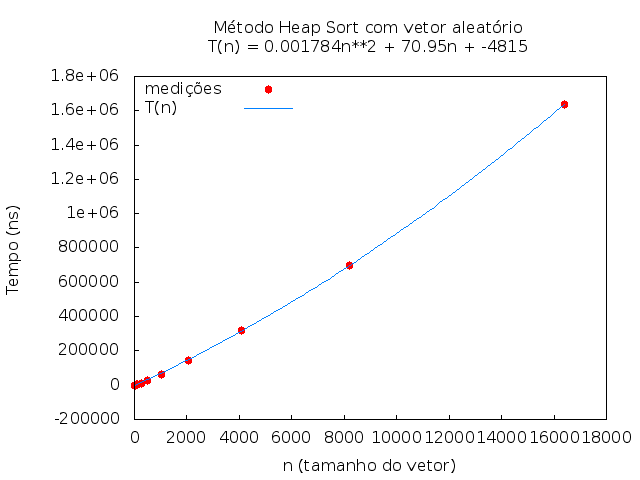
\includegraphics[width=0.7\linewidth]{graficos/HeapSort/vIntAleatorio/vIntAleatorio.png}
  \caption{Corte Haste Bottom Up - Vetor Crescente P40}
\end{figure}




\subsection{Vetor Crescente P50}
Tabela gerada utilizando Corte Haste Bottom Up com vetores de tamanho n, sendo n = $(2^k)$, de k = 4..14 e inseridos de forma crescente P50.
\begin{table}[H]
\centering
\caption{Corte Haste Bottom Up com Vetor Crescente P50}
\label{my-label}
\begin{tabular}{|l|l|}
\hline
\multicolumn{1}{|c|}{\textbf{Número de Elementos}} & \multicolumn{1}{c|}{\textbf{Tempo de execução em nanosegundos}} \\ \hline
16 & 599 \\ \hline
32 & 913 \\ \hline
64 & 1798 \\ \hline
128 & 4618 \\ \hline
256 & 14530 \\ \hline
512 & 51214 \\ \hline
1024 & 193794 \\ \hline
2048 & 761470 \\ \hline
4096 & 2965012 \\ \hline
8192 & 12774326 \\ \hline
16384 & 48066532 \\ \hline
\end{tabular}
\end{table}

\begin{figure}[H]
    \centering
    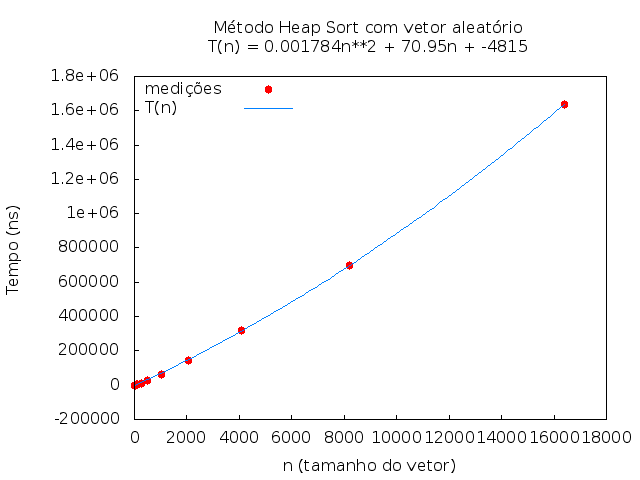
\includegraphics[width=0.7\linewidth]{graficos/HeapSort/vIntAleatorio/vIntAleatorio.png}
  \caption{Corte Haste Bottom Up - Vetor Crescente P50}
\end{figure}







\subsection{Vetor Decrescente}
Tabela gerada utilizando Corte Haste Bottom Up com vetores de tamanho n, sendo n = $(2^k)$, de k = 4..14 e inseridos de forma decrescente.
\begin{table}[H]
\centering
\caption{Corte Haste Bottom Up com Vetor Decrescente}
\label{my-label}
\begin{tabular}{|l|l|}
\hline
\multicolumn{1}{|c|}{\textbf{Número de Elementos}} & \multicolumn{1}{c|}{\textbf{Tempo de execução em nanosegundos}} \\ \hline
16 & 599 \\ \hline
32 & 913 \\ \hline
64 & 1798 \\ \hline
128 & 4618 \\ \hline
256 & 14530 \\ \hline
512 & 51214 \\ \hline
1024 & 193794 \\ \hline
2048 & 761470 \\ \hline
4096 & 2965012 \\ \hline
8192 & 12774326 \\ \hline
16384 & 48066532 \\ \hline
\end{tabular}
\end{table}

\begin{figure}[H]
    \centering
    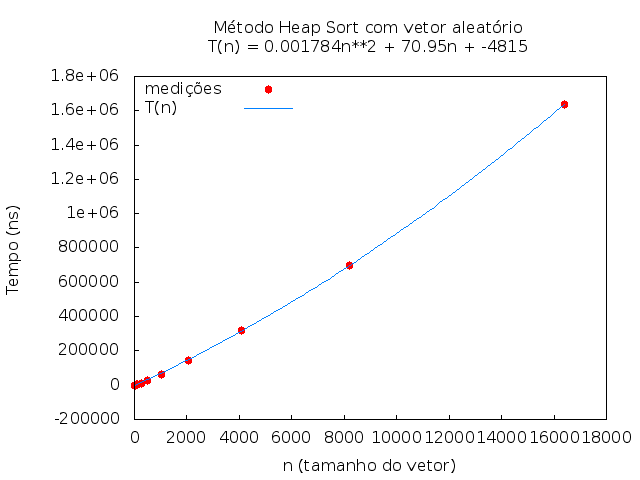
\includegraphics[width=0.7\linewidth]{graficos/HeapSort/vIntAleatorio/vIntAleatorio.png}
  \caption{Corte Haste Bottom Up - Vetor Decrescente}
\end{figure}





\subsection{Vetor Decrescente P10}
Tabela gerada utilizando Corte Haste Bottom Up com vetores de tamanho n, sendo n = $(2^k)$, de k = 4..14 e inseridos de forma decrescente P10.
\begin{table}[H]
\centering
\caption{Corte Haste Bottom Up com Vetor Decrescente P10}
\label{my-label}
\begin{tabular}{|l|l|}
\hline
\multicolumn{1}{|c|}{\textbf{Número de Elementos}} & \multicolumn{1}{c|}{\textbf{Tempo de execução em nanosegundos}} \\ \hline
16 & 599 \\ \hline
32 & 913 \\ \hline
64 & 1798 \\ \hline
128 & 4618 \\ \hline
256 & 14530 \\ \hline
512 & 51214 \\ \hline
1024 & 193794 \\ \hline
2048 & 761470 \\ \hline
4096 & 2965012 \\ \hline
8192 & 12774326 \\ \hline
16384 & 48066532 \\ \hline
\end{tabular}
\end{table}

\begin{figure}[H]
    \centering
    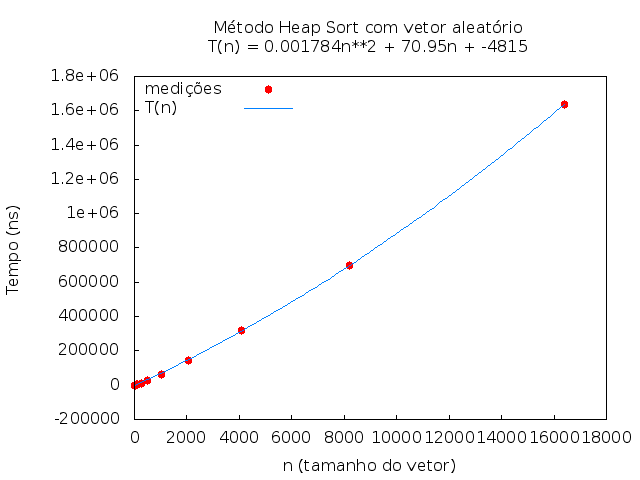
\includegraphics[width=0.7\linewidth]{graficos/HeapSort/vIntAleatorio/vIntAleatorio.png}
  \caption{Corte Haste Bottom Up - Vetor Decrescente P10}
\end{figure}




\subsection{Vetor Decrescente P20}
Tabela gerada utilizando Corte Haste Bottom Up com vetores de tamanho n, sendo n = $(2^k)$, de k = 4..14 e inseridos de forma decrescente P20.
\begin{table}[H]
\centering
\caption{Corte Haste Bottom Up com Vetor Decrescente P20}
\label{my-label}
\begin{tabular}{|l|l|}
\hline
\multicolumn{1}{|c|}{\textbf{Número de Elementos}} & \multicolumn{1}{c|}{\textbf{Tempo de execução em nanosegundos}} \\ \hline
16 & 599 \\ \hline
32 & 913 \\ \hline
64 & 1798 \\ \hline
128 & 4618 \\ \hline
256 & 14530 \\ \hline
512 & 51214 \\ \hline
1024 & 193794 \\ \hline
2048 & 761470 \\ \hline
4096 & 2965012 \\ \hline
8192 & 12774326 \\ \hline
16384 & 48066532 \\ \hline
\end{tabular}
\end{table}

\begin{figure}[H]
    \centering
    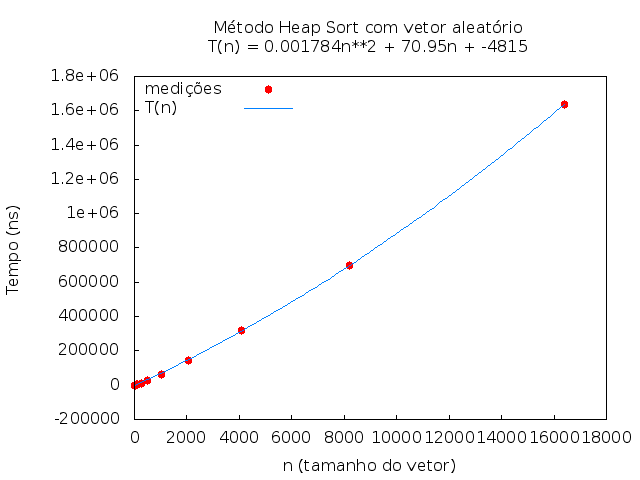
\includegraphics[width=0.7\linewidth]{graficos/HeapSort/vIntAleatorio/vIntAleatorio.png}
  \caption{Corte Haste Bottom Up - Vetor Decrescente P20}
\end{figure}




\subsection{Vetor Decrescente P30}
Tabela gerada utilizando Corte Haste Bottom Up com vetores de tamanho n, sendo n = $(2^k)$, de k = 4..14 e inseridos de forma decrescente P30.
\begin{table}[H]
\centering
\caption{Corte Haste Bottom Up com Vetor Decrescente P30}
\label{my-label}
\begin{tabular}{|l|l|}
\hline
\multicolumn{1}{|c|}{\textbf{Número de Elementos}} & \multicolumn{1}{c|}{\textbf{Tempo de execução em nanosegundos}} \\ \hline
16 & 599 \\ \hline
32 & 913 \\ \hline
64 & 1798 \\ \hline
128 & 4618 \\ \hline
256 & 14530 \\ \hline
512 & 51214 \\ \hline
1024 & 193794 \\ \hline
2048 & 761470 \\ \hline
4096 & 2965012 \\ \hline
8192 & 12774326 \\ \hline
16384 & 48066532 \\ \hline
\end{tabular}
\end{table}

\begin{figure}[H]
    \centering
    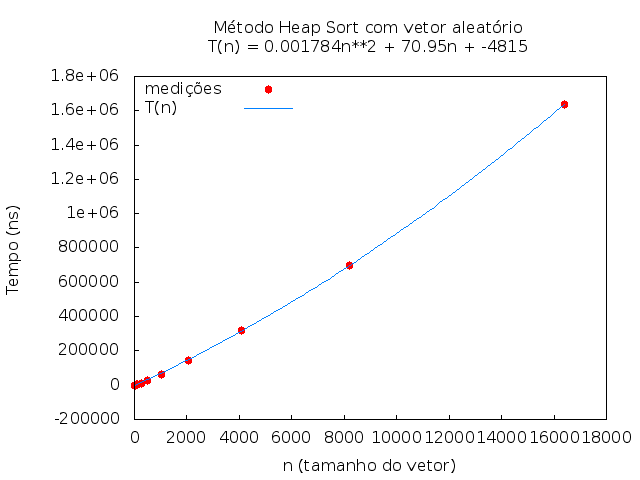
\includegraphics[width=0.7\linewidth]{graficos/HeapSort/vIntAleatorio/vIntAleatorio.png}
  \caption{Corte Haste Bottom Up - Vetor Decrescente P30}
\end{figure}





\subsection{Vetor Decrescente P40}
Tabela gerada utilizando Corte Haste Bottom Up com vetores de tamanho n, sendo n = $(2^k)$, de k = 4..14 e inseridos de forma decrescente P40.
\begin{table}[H]
\centering
\caption{Corte Haste Bottom Up com Vetor Decrescente P40}
\label{my-label}
\begin{tabular}{|l|l|}
\hline
\multicolumn{1}{|c|}{\textbf{Número de Elementos}} & \multicolumn{1}{c|}{\textbf{Tempo de execução em nanosegundos}} \\ \hline
16 & 599 \\ \hline
32 & 913 \\ \hline
64 & 1798 \\ \hline
128 & 4618 \\ \hline
256 & 14530 \\ \hline
512 & 51214 \\ \hline
1024 & 193794 \\ \hline
2048 & 761470 \\ \hline
4096 & 2965012 \\ \hline
8192 & 12774326 \\ \hline
16384 & 48066532 \\ \hline
\end{tabular}
\end{table}

\begin{figure}[H]
    \centering
    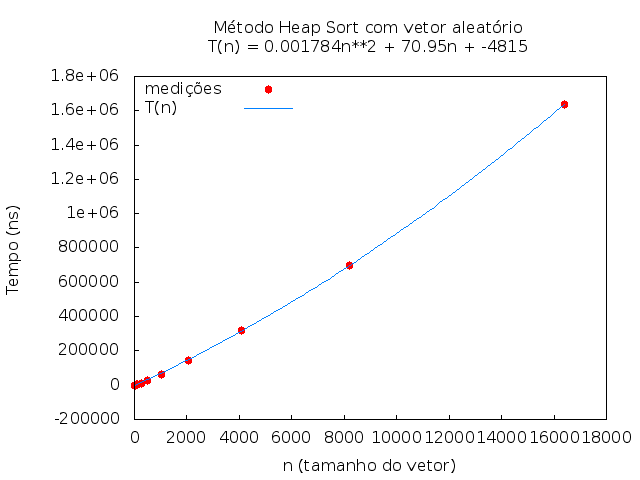
\includegraphics[width=0.7\linewidth]{graficos/HeapSort/vIntAleatorio/vIntAleatorio.png}
  \caption{Corte Haste Bottom Up - Vetor Decrescente P40}
\end{figure}





\subsection{Vetor Decrescente P50}
Tabela gerada utilizando Corte Haste Bottom Up com vetores de tamanho n, sendo n = $(2^k)$, de k = 4..14 e inseridos de forma decrescente P50.
\begin{table}[H]
\centering
\caption{Corte Haste Bottom Up com Vetor Decrescente P50}
\label{my-label}
\begin{tabular}{|l|l|}
\hline
\multicolumn{1}{|c|}{\textbf{Número de Elementos}} & \multicolumn{1}{c|}{\textbf{Tempo de execução em nanosegundos}} \\ \hline
16 & 599 \\ \hline
32 & 913 \\ \hline
64 & 1798 \\ \hline
128 & 4618 \\ \hline
256 & 14530 \\ \hline
512 & 51214 \\ \hline
1024 & 193794 \\ \hline
2048 & 761470 \\ \hline
4096 & 2965012 \\ \hline
8192 & 12774326 \\ \hline
16384 & 48066532 \\ \hline
\end{tabular}
\end{table}

\begin{figure}[H]
    \centering
    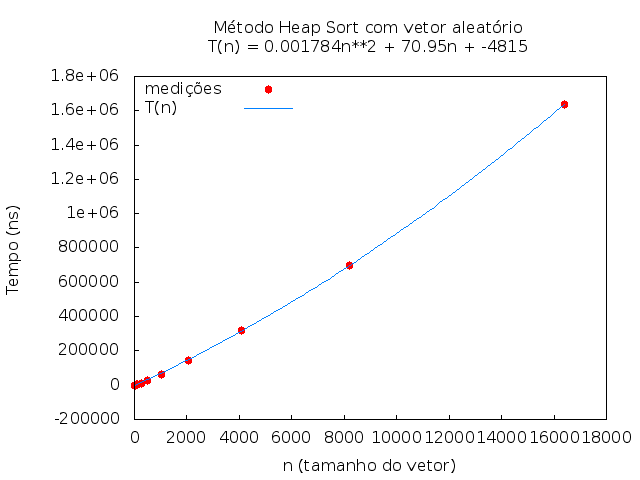
\includegraphics[width=0.7\linewidth]{graficos/HeapSort/vIntAleatorio/vIntAleatorio.png}
  \caption{Corte Haste Bottom Up - Vetor Decrescente P50}
\end{figure}




\section{Corte Haste Comum}

blablabal

Tabela gerada utilizando Corte Haste Comum com vetores de tamanho n, sendo n = $(2^k)$, de k = 4..14 e inseridos aleatóriamente, crescente, crescente P10, crescente P20, crescente P30, decrescente, decrescente P10, decrescente P20, decrescenteP30.
\begin{table}[H]
\centering
\caption{Corte Haste Bottom Up com vetor aleatório}
\label{my-label}
\begin{tabular}{|l|l|}
\hline
\multicolumn{1}{|c|}{\textbf{Número de Elementos}} & \multicolumn{1}{c|}{\textbf{Tempo de execução em nanosegundos}} \\ \hline
16 & 535410 \\ \hline
16 & 538372 \\ \hline
16 & 539477 \\ \hline
16 & 529753 \\ \hline
16 & 541344 \\ \hline
16 & 538372 \\ \hline
16 & 539477 \\ \hline
16 & 529753 \\ \hline
16 & 541344 \\ \hline
\end{tabular}
\end{table}

\begin{figure}[H]
    \centering
    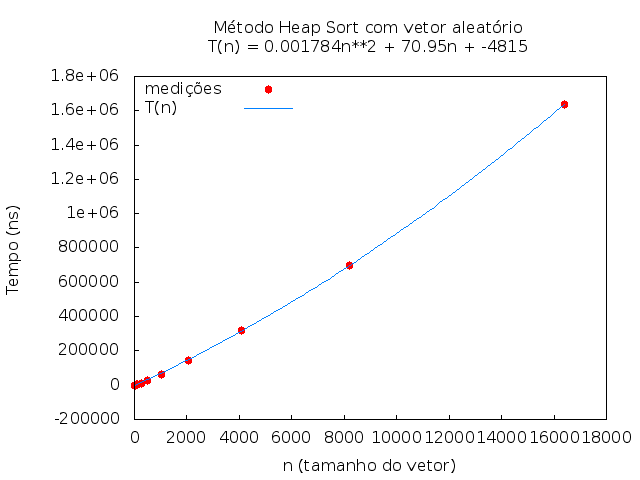
\includegraphics[width=0.7\linewidth]{graficos/HeapSort/vIntAleatorio/vIntAleatorio.png}
  \caption{Corte Haste Comum}
\end{figure}







\section{Corte Haste Memoizada}

blablbablabla

\subsection{Vetor aleatorio}
Tabela gerada utilizando Corte Haste Memoizada com vetores de tamanho n, sendo n = $(2^k)$, de k = 4..14 e inseridos aleatóriamente.
\begin{table}[H]
\centering
\caption{Corte Haste Memoizada com vetor aleatório}
\label{my-label}
\begin{tabular}{|l|l|}
\hline
\multicolumn{1}{|c|}{\textbf{Número de Elementos}} & \multicolumn{1}{c|}{\textbf{Tempo de execução em nanosegundos}} \\ \hline
16 & 357 \\ \hline
32 & 362 \\ \hline
64 & 364 \\ \hline
128 & 372 \\ \hline
256 & 392 \\ \hline
512 & 427 \\ \hline
1024 & 545 \\ \hline
2048 & 604 \\ \hline
4096 & 1085 \\ \hline
8192 & 13662 \\ \hline
16384 & 6253 \\ \hline
\end{tabular}
\end{table}

\begin{figure}[H]
    \centering
    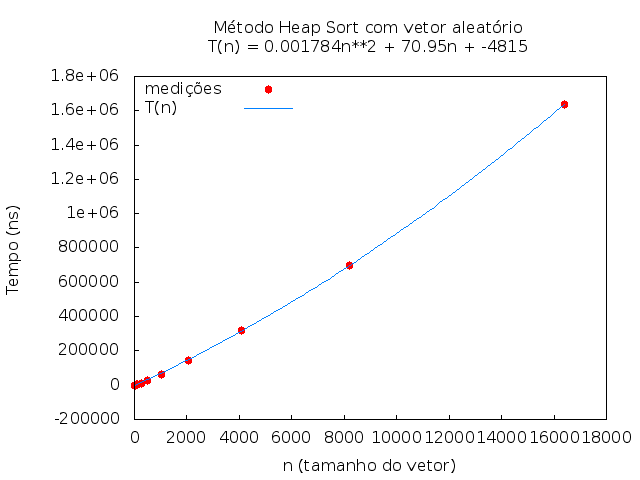
\includegraphics[width=0.7\linewidth]{graficos/HeapSort/vIntAleatorio/vIntAleatorio.png}
  \caption{Corte Haste Memoizada - Vetor Aleatório}
\end{figure}



\subsection{Vetor Crescente}
Tabela gerada utilizando Corte Haste Memoizada com vetores de tamanho n, sendo n = $(2^k)$, de k = 4..14 e inseridos de forma crescente.
\begin{table}[H]
\centering
\caption{Corte Haste Memoizada com Vetor Crescente}
\label{my-label}
\begin{tabular}{|l|l|}
\hline
\multicolumn{1}{|c|}{\textbf{Número de Elementos}} & \multicolumn{1}{c|}{\textbf{Tempo de execução em nanosegundos}} \\ \hline
16 & 357 \\ \hline
32 & 362 \\ \hline
64 & 364 \\ \hline
128 & 372 \\ \hline
256 & 392 \\ \hline
512 & 427 \\ \hline
1024 & 545 \\ \hline
2048 & 604 \\ \hline
4096 & 1085 \\ \hline
8192 & 13662 \\ \hline
16384 & 6253 \\ \hline
\end{tabular}
\end{table}

\begin{figure}[H]
    \centering
    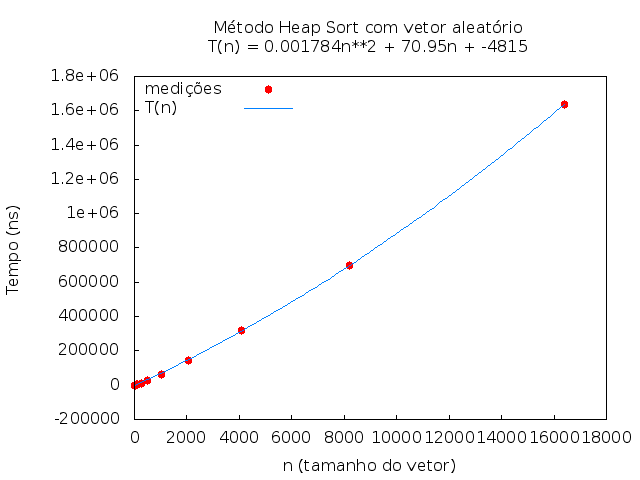
\includegraphics[width=0.7\linewidth]{graficos/HeapSort/vIntAleatorio/vIntAleatorio.png}
  \caption{Corte Haste Memoizada - Vetor Crescente}
\end{figure}






\subsection{Vetor Crescente P10}
Tabela gerada utilizando Corte Haste Memoizada com vetores de tamanho n, sendo n = $(2^k)$, de k = 4..14 e inseridos de forma crescente P10.
\begin{table}[H]
\centering
\caption{Corte Haste Memoizada com Vetor Crescente P10}
\label{my-label}
\begin{tabular}{|l|l|}
\hline
\multicolumn{1}{|c|}{\textbf{Número de Elementos}} & \multicolumn{1}{c|}{\textbf{Tempo de execução em nanosegundos}} \\ \hline
16 & 357 \\ \hline
32 & 362 \\ \hline
64 & 364 \\ \hline
128 & 372 \\ \hline
256 & 392 \\ \hline
512 & 427 \\ \hline
1024 & 545 \\ \hline
2048 & 604 \\ \hline
4096 & 1085 \\ \hline
8192 & 13662 \\ \hline
16384 & 6253 \\ \hline
\end{tabular}
\end{table}

\begin{figure}[H]
    \centering
    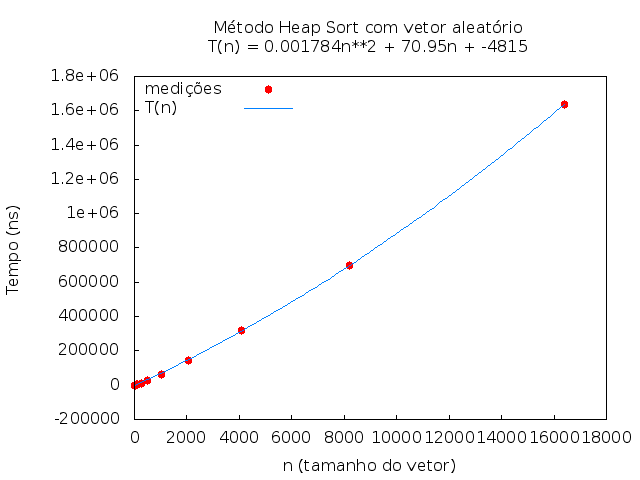
\includegraphics[width=0.7\linewidth]{graficos/HeapSort/vIntAleatorio/vIntAleatorio.png}
  \caption{Corte Haste Memoizada - Vetor Crescente P10}
\end{figure}





\subsection{Vetor Crescente P20}
Tabela gerada utilizando Corte Haste Memoizada com vetores de tamanho n, sendo n = $(2^k)$, de k = 4..14 e inseridos de forma crescente P20.
\begin{table}[H]
\centering
\caption{Corte Haste Memoizada com Vetor Crescente P20}
\label{my-label}
\begin{tabular}{|l|l|}
\hline
\multicolumn{1}{|c|}{\textbf{Número de Elementos}} & \multicolumn{1}{c|}{\textbf{Tempo de execução em nanosegundos}} \\ \hline
16 & 357 \\ \hline
32 & 362 \\ \hline
64 & 364 \\ \hline
128 & 372 \\ \hline
256 & 392 \\ \hline
512 & 427 \\ \hline
1024 & 545 \\ \hline
2048 & 604 \\ \hline
4096 & 1085 \\ \hline
8192 & 13662 \\ \hline
16384 & 6253 \\ \hline
\end{tabular}
\end{table}

\begin{figure}[H]
    \centering
    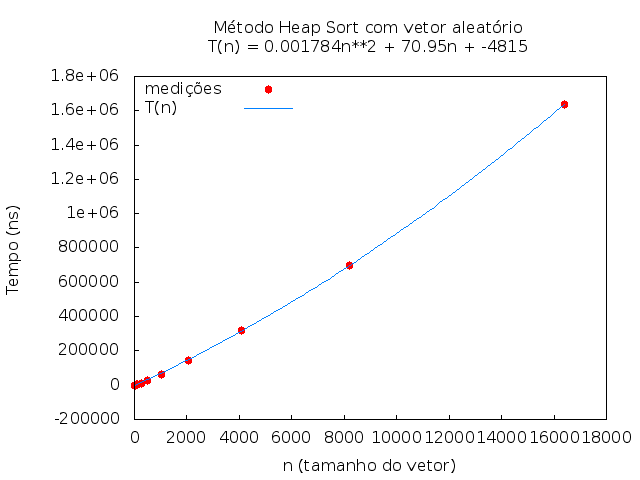
\includegraphics[width=0.7\linewidth]{graficos/HeapSort/vIntAleatorio/vIntAleatorio.png}
  \caption{Corte Haste Memoizada - Vetor Crescente P20}
\end{figure}



\subsection{Vetor Crescente P30}
Tabela gerada utilizando Corte Haste Memoizada com vetores de tamanho n, sendo n = $(2^k)$, de k = 4..14 e inseridos de forma crescente P30.
\begin{table}[H]
\centering
\caption{Corte Haste Memoizada com Vetor Crescente P30}
\label{my-label}
\begin{tabular}{|l|l|}
\hline
\multicolumn{1}{|c|}{\textbf{Número de Elementos}} & \multicolumn{1}{c|}{\textbf{Tempo de execução em nanosegundos}} \\ \hline
16 & 357 \\ \hline
32 & 362 \\ \hline
64 & 364 \\ \hline
128 & 372 \\ \hline
256 & 392 \\ \hline
512 & 427 \\ \hline
1024 & 545 \\ \hline
2048 & 604 \\ \hline
4096 & 1085 \\ \hline
8192 & 13662 \\ \hline
16384 & 6253 \\ \hline
\end{tabular}
\end{table}

\begin{figure}[H]
    \centering
    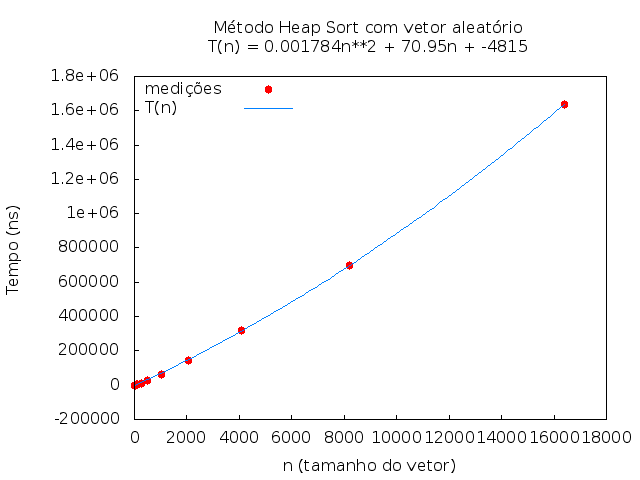
\includegraphics[width=0.7\linewidth]{graficos/HeapSort/vIntAleatorio/vIntAleatorio.png}
  \caption{Corte Haste Memoizada - Vetor Crescente P30}
\end{figure}





\subsection{Vetor Crescente P40}
Tabela gerada utilizando Corte Haste Memoizada com vetores de tamanho n, sendo n = $(2^k)$, de k = 4..14 e inseridos de forma crescente P40.
\begin{table}[H]
\centering
\caption{Corte Haste Memoizada com Vetor Crescente P40}
\label{my-label}
\begin{tabular}{|l|l|}
\hline
\multicolumn{1}{|c|}{\textbf{Número de Elementos}} & \multicolumn{1}{c|}{\textbf{Tempo de execução em nanosegundos}} \\ \hline
16 & 357 \\ \hline
32 & 362 \\ \hline
64 & 364 \\ \hline
128 & 372 \\ \hline
256 & 392 \\ \hline
512 & 427 \\ \hline
1024 & 545 \\ \hline
2048 & 604 \\ \hline
4096 & 1085 \\ \hline
8192 & 13662 \\ \hline
16384 & 6253 \\ \hline
\end{tabular}
\end{table}

\begin{figure}[H]
    \centering
    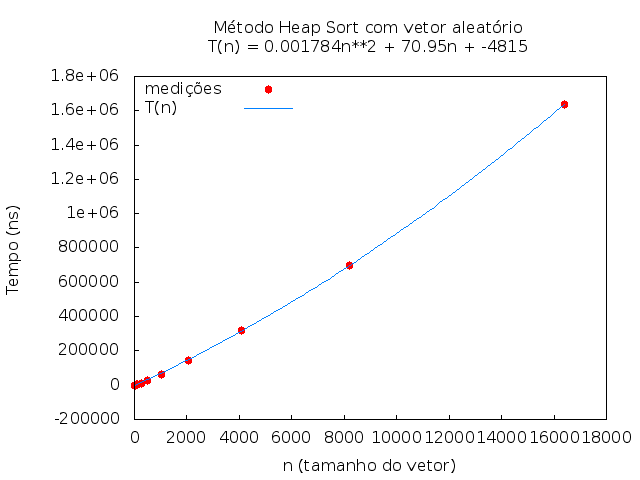
\includegraphics[width=0.7\linewidth]{graficos/HeapSort/vIntAleatorio/vIntAleatorio.png}
  \caption{Corte Haste Memoizada - Vetor Crescente P40}
\end{figure}




\subsection{Vetor Crescente P50}
Tabela gerada utilizando Corte Haste Memoizada com vetores de tamanho n, sendo n = $(2^k)$, de k = 4..14 e inseridos de forma crescente P50.
\begin{table}[H]
\centering
\caption{Corte Haste Memoizada com Vetor Crescente P50}
\label{my-label}
\begin{tabular}{|l|l|}
\hline
\multicolumn{1}{|c|}{\textbf{Número de Elementos}} & \multicolumn{1}{c|}{\textbf{Tempo de execução em nanosegundos}} \\ \hline
16 & 357 \\ \hline
32 & 362 \\ \hline
64 & 364 \\ \hline
128 & 372 \\ \hline
256 & 392 \\ \hline
512 & 427 \\ \hline
1024 & 545 \\ \hline
2048 & 604 \\ \hline
4096 & 1085 \\ \hline
8192 & 13662 \\ \hline
16384 & 6253 \\ \hline
\end{tabular}
\end{table}

\begin{figure}[H]
    \centering
    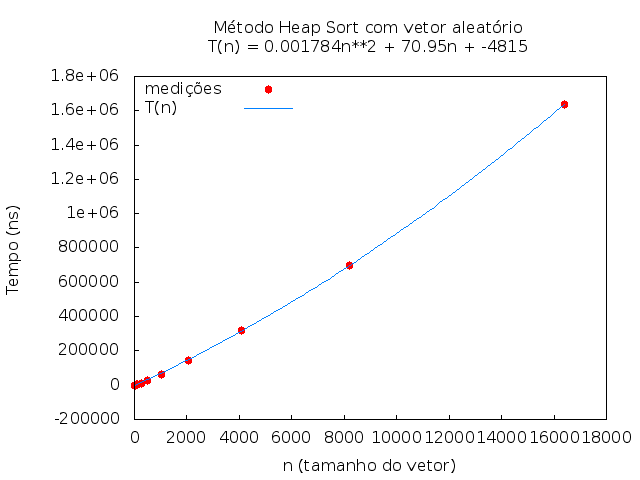
\includegraphics[width=0.7\linewidth]{graficos/HeapSort/vIntAleatorio/vIntAleatorio.png}
  \caption{Corte Haste Memoizada - Vetor Crescente P50}
\end{figure}




\subsection{Vetor Decrescente}
Tabela gerada utilizando Corte Haste Memoizada com vetores de tamanho n, sendo n = $(2^k)$, de k = 4..14 e inseridos de forma decrescente.
\begin{table}[H]
\centering
\caption{Corte Haste Memoizada com Vetor Decrescente}
\label{my-label}
\begin{tabular}{|l|l|}
\hline
\multicolumn{1}{|c|}{\textbf{Número de Elementos}} & \multicolumn{1}{c|}{\textbf{Tempo de execução em nanosegundos}} \\ \hline
16 & 357 \\ \hline
32 & 362 \\ \hline
64 & 364 \\ \hline
128 & 372 \\ \hline
256 & 392 \\ \hline
512 & 427 \\ \hline
1024 & 545 \\ \hline
2048 & 604 \\ \hline
4096 & 1085 \\ \hline
8192 & 13662 \\ \hline
16384 & 6253 \\ \hline
\end{tabular}
\end{table}

\begin{figure}[H]
    \centering
    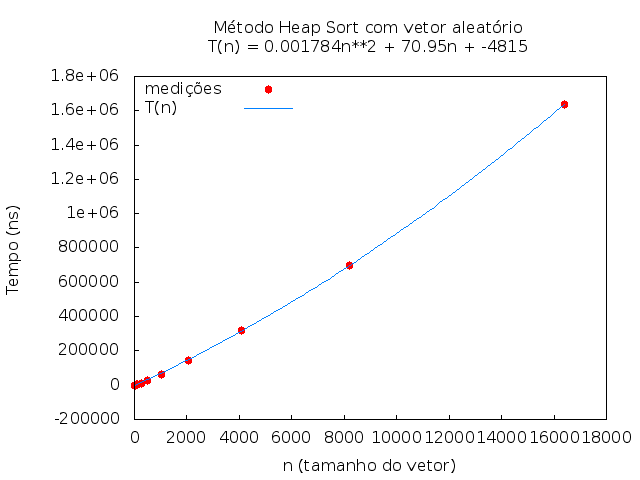
\includegraphics[width=0.7\linewidth]{graficos/HeapSort/vIntAleatorio/vIntAleatorio.png}
  \caption{Corte Haste Memoizada - Vetor Decrescente}
\end{figure}



\subsection{Vetor Decrescente P10}
Tabela gerada utilizando Corte Haste Memoizada com vetores de tamanho n, sendo n = $(2^k)$, de k = 4..14 e inseridos de forma decrescente P10.
\begin{table}[H]
\centering
\caption{Corte Haste Memoizada com Vetor Decrescente P10}
\label{my-label}
\begin{tabular}{|l|l|}
\hline
\multicolumn{1}{|c|}{\textbf{Número de Elementos}} & \multicolumn{1}{c|}{\textbf{Tempo de execução em nanosegundos}} \\ \hline
16 & 357 \\ \hline
32 & 362 \\ \hline
64 & 364 \\ \hline
128 & 372 \\ \hline
256 & 392 \\ \hline
512 & 427 \\ \hline
1024 & 545 \\ \hline
2048 & 604 \\ \hline
4096 & 1085 \\ \hline
8192 & 13662 \\ \hline
16384 & 6253 \\ \hline
\end{tabular}
\end{table}

\begin{figure}[H]
    \centering
    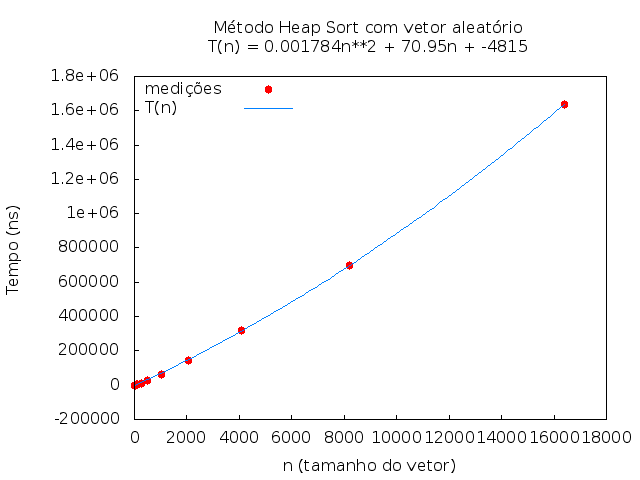
\includegraphics[width=0.7\linewidth]{graficos/HeapSort/vIntAleatorio/vIntAleatorio.png}
  \caption{Corte Haste Memoizada - Vetor Decrescente P10}
\end{figure}





\subsection{Vetor Decrescente P20}
Tabela gerada utilizando Corte Haste Memoizada com vetores de tamanho n, sendo n = $(2^k)$, de k = 4..14 e inseridos de forma decrescente P20.
\begin{table}[H]
\centering
\caption{Corte Haste Memoizada com Vetor Decrescente P20}
\label{my-label}
\begin{tabular}{|l|l|}
\hline
\multicolumn{1}{|c|}{\textbf{Número de Elementos}} & \multicolumn{1}{c|}{\textbf{Tempo de execução em nanosegundos}} \\ \hline
16 & 357 \\ \hline
32 & 362 \\ \hline
64 & 364 \\ \hline
128 & 372 \\ \hline
256 & 392 \\ \hline
512 & 427 \\ \hline
1024 & 545 \\ \hline
2048 & 604 \\ \hline
4096 & 1085 \\ \hline
8192 & 13662 \\ \hline
16384 & 6253 \\ \hline
\end{tabular}
\end{table}

\begin{figure}[H]
    \centering
    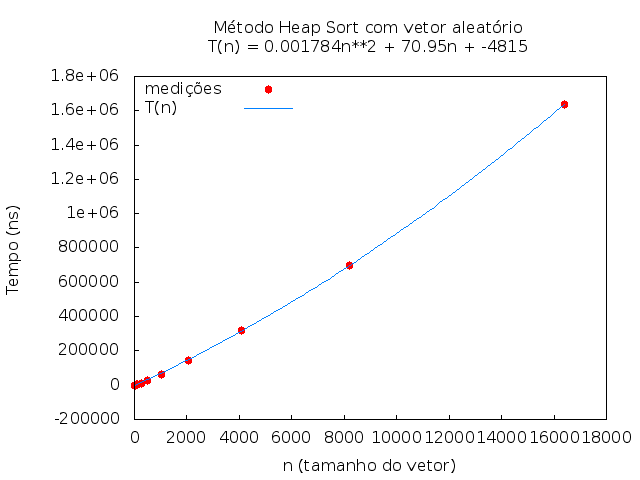
\includegraphics[width=0.7\linewidth]{graficos/HeapSort/vIntAleatorio/vIntAleatorio.png}
  \caption{Corte Haste Memoizada - Vetor Decrescente P20}
\end{figure}



\subsection{Vetor Decrescente P30}
Tabela gerada utilizando Corte Haste Memoizada com vetores de tamanho n, sendo n = $(2^k)$, de k = 4..14 e inseridos de forma decrescente P30.
\begin{table}[H]
\centering
\caption{Corte Haste Memoizada com Vetor Decrescente P30}
\label{my-label}
\begin{tabular}{|l|l|}
\hline
\multicolumn{1}{|c|}{\textbf{Número de Elementos}} & \multicolumn{1}{c|}{\textbf{Tempo de execução em nanosegundos}} \\ \hline
16 & 357 \\ \hline
32 & 362 \\ \hline
64 & 364 \\ \hline
128 & 372 \\ \hline
256 & 392 \\ \hline
512 & 427 \\ \hline
1024 & 545 \\ \hline
2048 & 604 \\ \hline
4096 & 1085 \\ \hline
8192 & 13662 \\ \hline
16384 & 6253 \\ \hline
\end{tabular}
\end{table}

\begin{figure}[H]
    \centering
    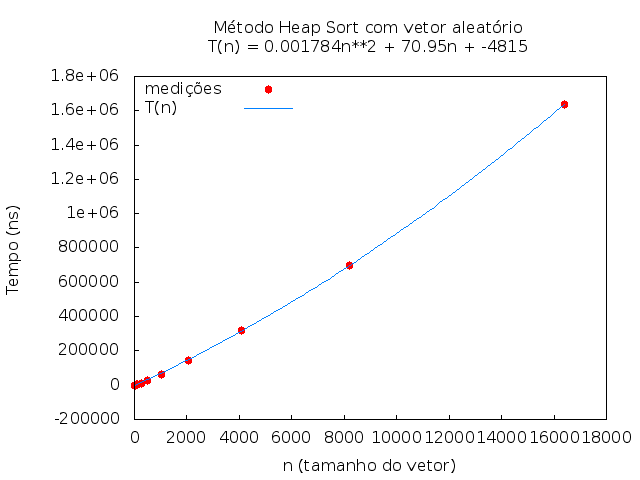
\includegraphics[width=0.7\linewidth]{graficos/HeapSort/vIntAleatorio/vIntAleatorio.png}
  \caption{Corte Haste Memoizada - Vetor Decrescente P30}
\end{figure}




\subsection{Vetor Decrescente P40}
Tabela gerada utilizando Corte Haste Memoizada com vetores de tamanho n, sendo n = $(2^k)$, de k = 4..14 e inseridos de forma decrescente P40.
\begin{table}[H]
\centering
\caption{Corte Haste Memoizada com Vetor Decrescente P40}
\label{my-label}
\begin{tabular}{|l|l|}
\hline
\multicolumn{1}{|c|}{\textbf{Número de Elementos}} & \multicolumn{1}{c|}{\textbf{Tempo de execução em nanosegundos}} \\ \hline
16 & 357 \\ \hline
32 & 362 \\ \hline
64 & 364 \\ \hline
128 & 372 \\ \hline
256 & 392 \\ \hline
512 & 427 \\ \hline
1024 & 545 \\ \hline
2048 & 604 \\ \hline
4096 & 1085 \\ \hline
8192 & 13662 \\ \hline
16384 & 6253 \\ \hline
\end{tabular}
\end{table}

\begin{figure}[H]
    \centering
    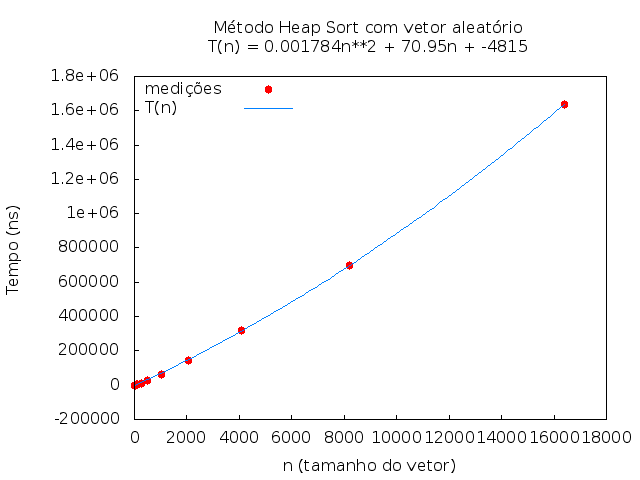
\includegraphics[width=0.7\linewidth]{graficos/HeapSort/vIntAleatorio/vIntAleatorio.png}
  \caption{Corte Haste Memoizada - Vetor Decrescente P40}
\end{figure}





\subsection{Vetor Decrescente P50}
Tabela gerada utilizando Corte Haste Memoizada com vetores de tamanho n, sendo n = $(2^k)$, de k = 4..14 e inseridos de forma decrescente P50.
\begin{table}[H]
\centering
\caption{Corte Haste Memoizada com Vetor Decrescente P50}
\label{my-label}
\begin{tabular}{|l|l|}
\hline
\multicolumn{1}{|c|}{\textbf{Número de Elementos}} & \multicolumn{1}{c|}{\textbf{Tempo de execução em nanosegundos}} \\ \hline
16 & 357 \\ \hline
32 & 362 \\ \hline
64 & 364 \\ \hline
128 & 372 \\ \hline
256 & 392 \\ \hline
512 & 427 \\ \hline
1024 & 545 \\ \hline
2048 & 604 \\ \hline
4096 & 1085 \\ \hline
8192 & 13662 \\ \hline
16384 & 6253 \\ \hline
\end{tabular}
\end{table}

\begin{figure}[H]
    \centering
    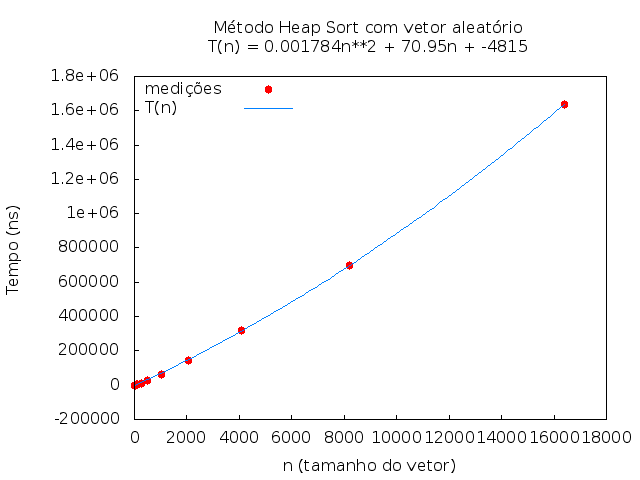
\includegraphics[width=0.7\linewidth]{graficos/HeapSort/vIntAleatorio/vIntAleatorio.png}
  \caption{Corte Haste Memoizada - Vetor Decrescente P50}
\end{figure}



\section{Parentização Bottom Up}

bLABLABALBALBAL

\subsection{Vetor aleatorio}
Tabela gerada utilizando Parentização Bottom Up com vetores de tamanho n, sendo n = $(2^k)$, de k = 4..14 e inseridos aleatóriamente.
\begin{table}[H]
\centering
\caption{Parentização Bottom Up com vetor aleatório}
\label{my-label}
\begin{tabular}{|l|l|}
\hline
\multicolumn{1}{|c|}{\textbf{Número de Elementos}} & \multicolumn{1}{c|}{\textbf{Tempo de execução em nanosegundos}} \\ \hline
16 & 8230 \\ \hline
32 & 19874 \\ \hline
64 & 138865 \\ \hline
128 & 1119535 \\ \hline
256 & 7674247 \\ \hline
512 & 70240583 \\ \hline
1024 & 1582607779 \\ \hline
\end{tabular}
\end{table}

\begin{figure}[H]
    \centering
    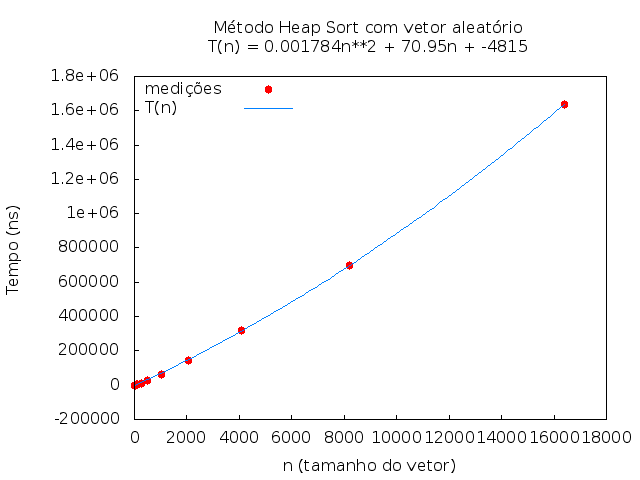
\includegraphics[width=0.7\linewidth]{graficos/HeapSort/vIntAleatorio/vIntAleatorio.png}
  \caption{Parentização Bottom Up - Vetor Aleatório}
\end{figure}



\subsection{Vetor Crescente}
Tabela gerada utilizando Parentização Bottom Up com vetores de tamanho n, sendo n = $(2^k)$, de k = 4..14 e inseridos Crescente.
\begin{table}[H]
\centering
\caption{Parentização Bottom Up com vetor Crescente}
\label{my-label}
\begin{tabular}{|l|l|}
\hline
\multicolumn{1}{|c|}{\textbf{Número de Elementos}} & \multicolumn{1}{c|}{\textbf{Tempo de execução em nanosegundos}} \\ \hline
16 & 8230 \\ \hline
32 & 19874 \\ \hline
64 & 138865 \\ \hline
128 & 1119535 \\ \hline
256 & 7674247 \\ \hline
512 & 70240583 \\ \hline
1024 & 1582607779 \\ \hline
\end{tabular}
\end{table}

\begin{figure}[H]
    \centering
    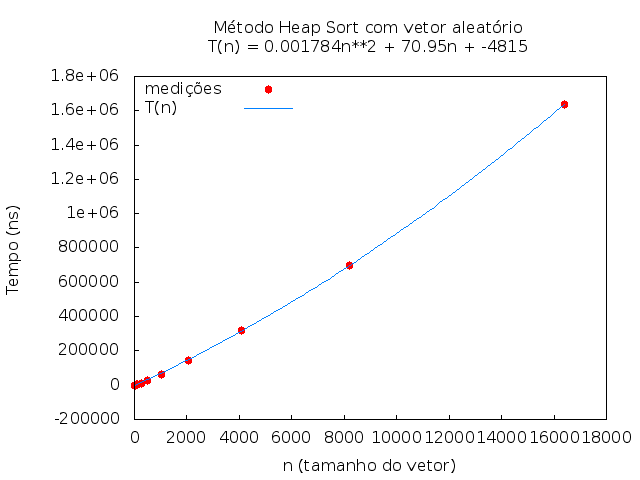
\includegraphics[width=0.7\linewidth]{graficos/HeapSort/vIntAleatorio/vIntAleatorio.png}
  \caption{Parentização Bottom Up - Vetor Crescente}
\end{figure}




\subsection{Vetor Crescente P10}
Tabela gerada utilizando Parentização Bottom Up com vetores de tamanho n, sendo n = $(2^k)$, de k = 4..14 e inseridos Crescente P10.
\begin{table}[H]
\centering
\caption{Parentização Bottom Up com vetor Crescente P10}
\label{my-label}
\begin{tabular}{|l|l|}
\hline
\multicolumn{1}{|c|}{\textbf{Número de Elementos}} & \multicolumn{1}{c|}{\textbf{Tempo de execução em nanosegundos}} \\ \hline
16 & 8230 \\ \hline
32 & 19874 \\ \hline
64 & 138865 \\ \hline
128 & 1119535 \\ \hline
256 & 7674247 \\ \hline
512 & 70240583 \\ \hline
1024 & 1582607779 \\ \hline
\end{tabular}
\end{table}

\begin{figure}[H]
    \centering
    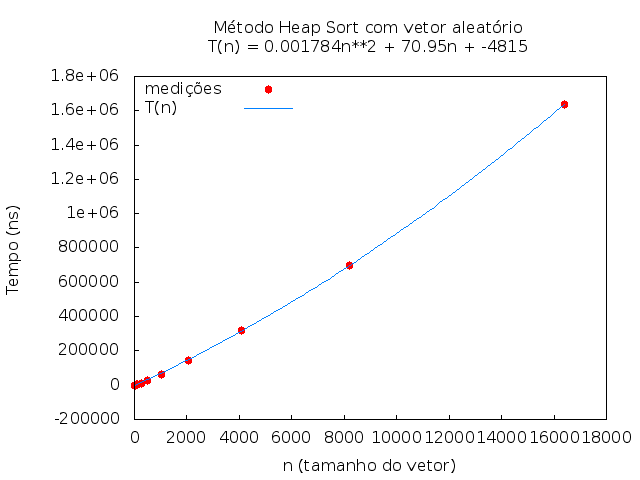
\includegraphics[width=0.7\linewidth]{graficos/HeapSort/vIntAleatorio/vIntAleatorio.png}
  \caption{Parentização Bottom Up - Vetor Crescente P10}
\end{figure}




\subsection{Vetor Crescente P20}
Tabela gerada utilizando Parentização Bottom Up com vetores de tamanho n, sendo n = $(2^k)$, de k = 4..14 e inseridos Crescente P20.
\begin{table}[H]
\centering
\caption{Parentização Bottom Up com vetor Crescente P20}
\label{my-label}
\begin{tabular}{|l|l|}
\hline
\multicolumn{1}{|c|}{\textbf{Número de Elementos}} & \multicolumn{1}{c|}{\textbf{Tempo de execução em nanosegundos}} \\ \hline
16 & 8230 \\ \hline
32 & 19874 \\ \hline
64 & 138865 \\ \hline
128 & 1119535 \\ \hline
256 & 7674247 \\ \hline
512 & 70240583 \\ \hline
1024 & 1582607779 \\ \hline
\end{tabular}
\end{table}

\begin{figure}[H]
    \centering
    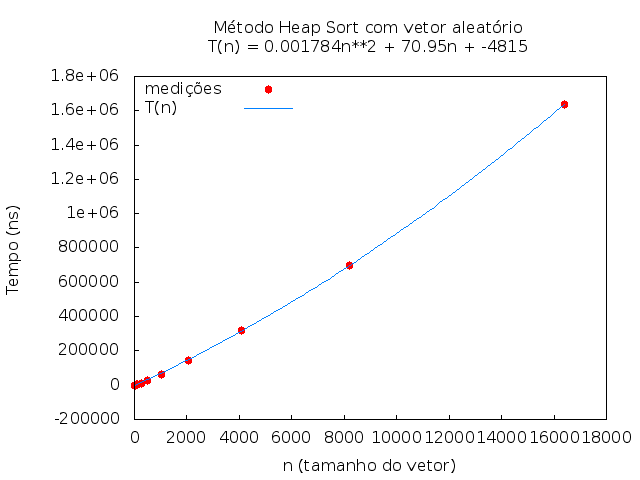
\includegraphics[width=0.7\linewidth]{graficos/HeapSort/vIntAleatorio/vIntAleatorio.png}
  \caption{Parentização Bottom Up - Vetor Crescente P20}
\end{figure}




\subsection{Vetor Crescente P30}
Tabela gerada utilizando Parentização Bottom Up com vetores de tamanho n, sendo n = $(2^k)$, de k = 4..14 e inseridos Crescente P30.
\begin{table}[H]
\centering
\caption{Parentização Bottom Up com vetor Crescente P30}
\label{my-label}
\begin{tabular}{|l|l|}
\hline
\multicolumn{1}{|c|}{\textbf{Número de Elementos}} & \multicolumn{1}{c|}{\textbf{Tempo de execução em nanosegundos}} \\ \hline
16 & 8230 \\ \hline
32 & 19874 \\ \hline
64 & 138865 \\ \hline
128 & 1119535 \\ \hline
256 & 7674247 \\ \hline
512 & 70240583 \\ \hline
1024 & 1582607779 \\ \hline
\end{tabular}
\end{table}

\begin{figure}[H]
    \centering
    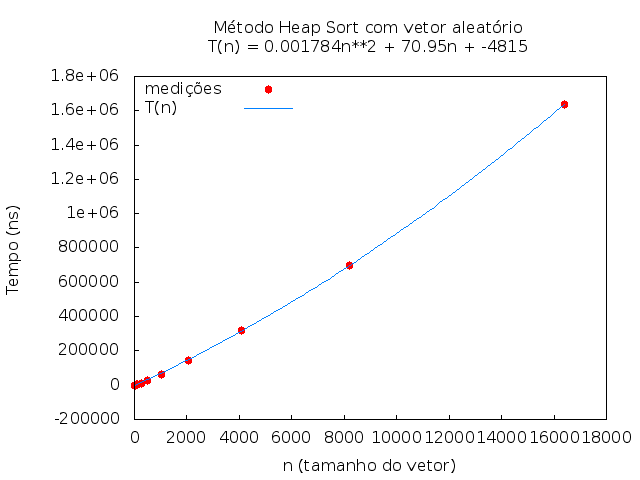
\includegraphics[width=0.7\linewidth]{graficos/HeapSort/vIntAleatorio/vIntAleatorio.png}
  \caption{Parentização Bottom Up - Vetor Crescente P30}
\end{figure}



\subsection{Vetor Crescente P40}
Tabela gerada utilizando Parentização Bottom Up com vetores de tamanho n, sendo n = $(2^k)$, de k = 4..14 e inseridos Crescente P40.
\begin{table}[H]
\centering
\caption{Parentização Bottom Up com vetor Crescente P40}
\label{my-label}
\begin{tabular}{|l|l|}
\hline
\multicolumn{1}{|c|}{\textbf{Número de Elementos}} & \multicolumn{1}{c|}{\textbf{Tempo de execução em nanosegundos}} \\ \hline
16 & 8230 \\ \hline
32 & 19874 \\ \hline
64 & 138865 \\ \hline
128 & 1119535 \\ \hline
256 & 7674247 \\ \hline
512 & 70240583 \\ \hline
1024 & 1582607779 \\ \hline
\end{tabular}
\end{table}

\begin{figure}[H]
    \centering
    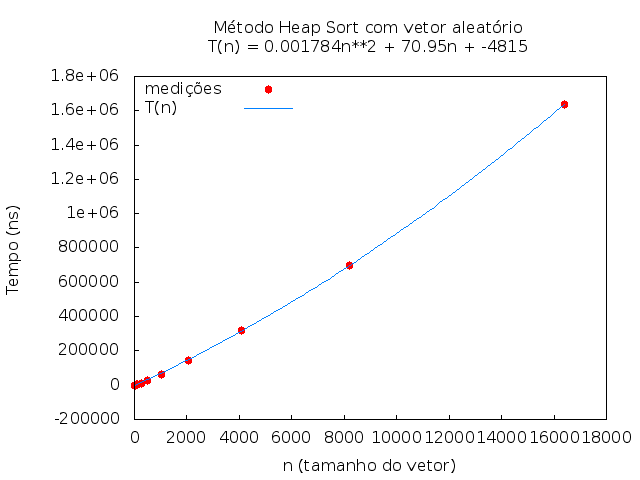
\includegraphics[width=0.7\linewidth]{graficos/HeapSort/vIntAleatorio/vIntAleatorio.png}
  \caption{Parentização Bottom Up - Vetor Crescente P40}
\end{figure}




\subsection{Vetor Crescente P50}
Tabela gerada utilizando Parentização Bottom Up com vetores de tamanho n, sendo n = $(2^k)$, de k = 4..14 e inseridos Crescente P50.
\begin{table}[H]
\centering
\caption{Parentização Bottom Up com vetor Crescente P50}
\label{my-label}
\begin{tabular}{|l|l|}
\hline
\multicolumn{1}{|c|}{\textbf{Número de Elementos}} & \multicolumn{1}{c|}{\textbf{Tempo de execução em nanosegundos}} \\ \hline
16 & 8230 \\ \hline
32 & 19874 \\ \hline
64 & 138865 \\ \hline
128 & 1119535 \\ \hline
256 & 7674247 \\ \hline
512 & 70240583 \\ \hline
1024 & 1582607779 \\ \hline
\end{tabular}
\end{table}

\begin{figure}[H]
    \centering
    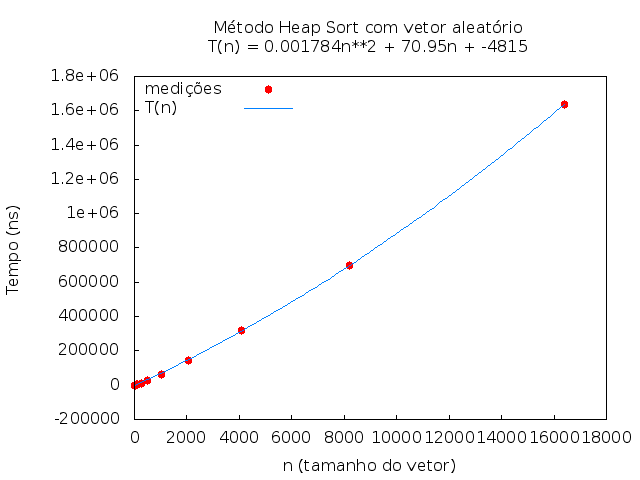
\includegraphics[width=0.7\linewidth]{graficos/HeapSort/vIntAleatorio/vIntAleatorio.png}
  \caption{Parentização Bottom Up - Vetor Crescente P50}
\end{figure}







\subsection{Vetor Decrescente}
Tabela gerada utilizando Parentização Bottom Up com vetores de tamanho n, sendo n = $(2^k)$, de k = 4..14 e inseridos Decrescente.
\begin{table}[H]
\centering
\caption{Parentização Bottom Up com vetor Decrescente}
\label{my-label}
\begin{tabular}{|l|l|}
\hline
\multicolumn{1}{|c|}{\textbf{Número de Elementos}} & \multicolumn{1}{c|}{\textbf{Tempo de execução em nanosegundos}} \\ \hline
16 & 8230 \\ \hline
32 & 19874 \\ \hline
64 & 138865 \\ \hline
128 & 1119535 \\ \hline
256 & 7674247 \\ \hline
512 & 70240583 \\ \hline
1024 & 1582607779 \\ \hline
\end{tabular}
\end{table}

\begin{figure}[H]
    \centering
    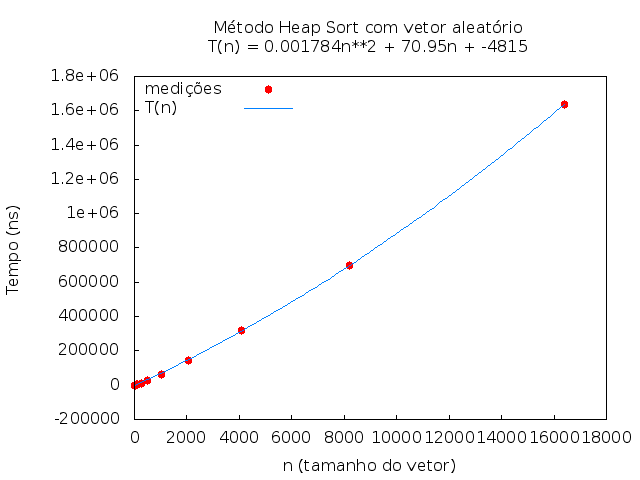
\includegraphics[width=0.7\linewidth]{graficos/HeapSort/vIntAleatorio/vIntAleatorio.png}
  \caption{Parentização Bottom Up - Vetor Decrescente}
\end{figure}




\subsection{Vetor Decrescente P10}
Tabela gerada utilizando Parentização Bottom Up com vetores de tamanho n, sendo n = $(2^k)$, de k = 4..14 e inseridos Decrescente P10.
\begin{table}[H]
\centering
\caption{Parentização Bottom Up com vetor Decrescente P10}
\label{my-label}
\begin{tabular}{|l|l|}
\hline
\multicolumn{1}{|c|}{\textbf{Número de Elementos}} & \multicolumn{1}{c|}{\textbf{Tempo de execução em nanosegundos}} \\ \hline
16 & 8230 \\ \hline
32 & 19874 \\ \hline
64 & 138865 \\ \hline
128 & 1119535 \\ \hline
256 & 7674247 \\ \hline
512 & 70240583 \\ \hline
1024 & 1582607779 \\ \hline
\end{tabular}
\end{table}

\begin{figure}[H]
    \centering
    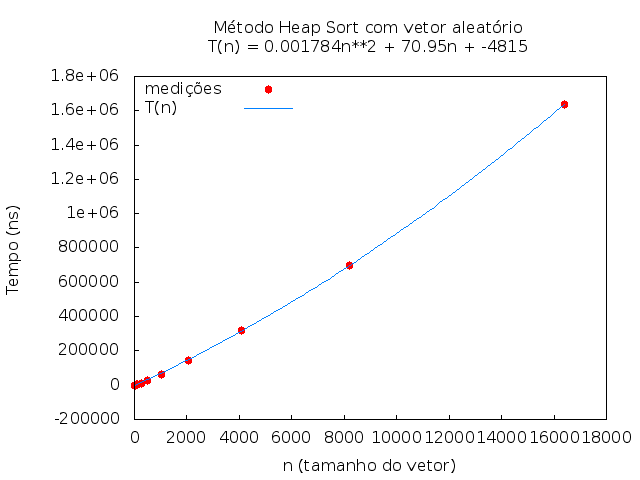
\includegraphics[width=0.7\linewidth]{graficos/HeapSort/vIntAleatorio/vIntAleatorio.png}
  \caption{Parentização Bottom Up - Vetor Decrescente P10}
\end{figure}





\subsection{Vetor Decrescente P20}
Tabela gerada utilizando Parentização Bottom Up com vetores de tamanho n, sendo n = $(2^k)$, de k = 4..14 e inseridos Decrescente P20.
\begin{table}[H]
\centering
\caption{Parentização Bottom Up com vetor Decrescente P20}
\label{my-label}
\begin{tabular}{|l|l|}
\hline
\multicolumn{1}{|c|}{\textbf{Número de Elementos}} & \multicolumn{1}{c|}{\textbf{Tempo de execução em nanosegundos}} \\ \hline
16 & 8230 \\ \hline
32 & 19874 \\ \hline
64 & 138865 \\ \hline
128 & 1119535 \\ \hline
256 & 7674247 \\ \hline
512 & 70240583 \\ \hline
1024 & 1582607779 \\ \hline
\end{tabular}
\end{table}

\begin{figure}[H]
    \centering
    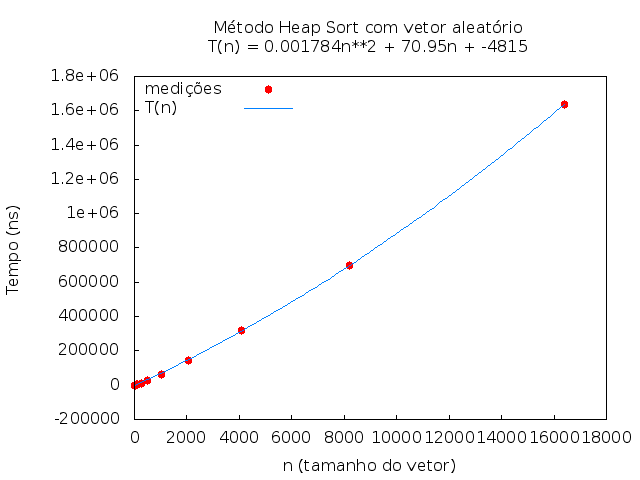
\includegraphics[width=0.7\linewidth]{graficos/HeapSort/vIntAleatorio/vIntAleatorio.png}
  \caption{Parentização Bottom Up - Vetor Decrescente P20}
\end{figure}




\subsection{Vetor Decrescente P30}
Tabela gerada utilizando Parentização Bottom Up com vetores de tamanho n, sendo n = $(2^k)$, de k = 4..14 e inseridos Decrescente P30.
\begin{table}[H]
\centering
\caption{Parentização Bottom Up com vetor Decrescente P30}
\label{my-label}
\begin{tabular}{|l|l|}
\hline
\multicolumn{1}{|c|}{\textbf{Número de Elementos}} & \multicolumn{1}{c|}{\textbf{Tempo de execução em nanosegundos}} \\ \hline
16 & 8230 \\ \hline
32 & 19874 \\ \hline
64 & 138865 \\ \hline
128 & 1119535 \\ \hline
256 & 7674247 \\ \hline
512 & 70240583 \\ \hline
1024 & 1582607779 \\ \hline
\end{tabular}
\end{table}

\begin{figure}[H]
    \centering
    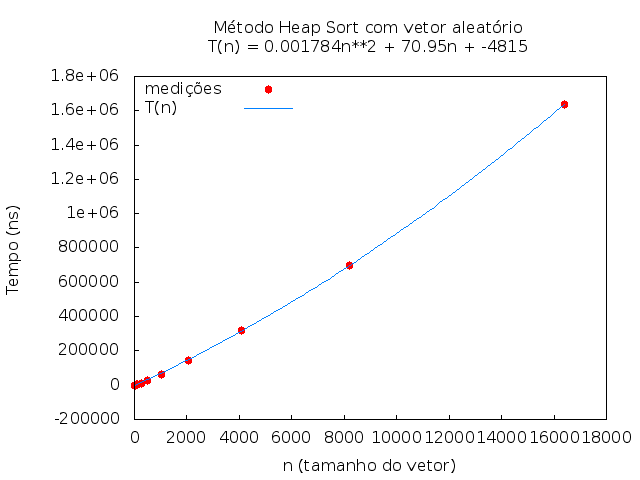
\includegraphics[width=0.7\linewidth]{graficos/HeapSort/vIntAleatorio/vIntAleatorio.png}
  \caption{Parentização Bottom Up - Vetor Decrescente P30}
\end{figure}





\subsection{Vetor Decrescente P40}
Tabela gerada utilizando Parentização Bottom Up com vetores de tamanho n, sendo n = $(2^k)$, de k = 4..14 e inseridos Decrescente P40.
\begin{table}[H]
\centering
\caption{Parentização Bottom Up com vetor Decrescente P40}
\label{my-label}
\begin{tabular}{|l|l|}
\hline
\multicolumn{1}{|c|}{\textbf{Número de Elementos}} & \multicolumn{1}{c|}{\textbf{Tempo de execução em nanosegundos}} \\ \hline
16 & 8230 \\ \hline
32 & 19874 \\ \hline
64 & 138865 \\ \hline
128 & 1119535 \\ \hline
256 & 7674247 \\ \hline
512 & 70240583 \\ \hline
1024 & 1582607779 \\ \hline
\end{tabular}
\end{table}

\begin{figure}[H]
    \centering
    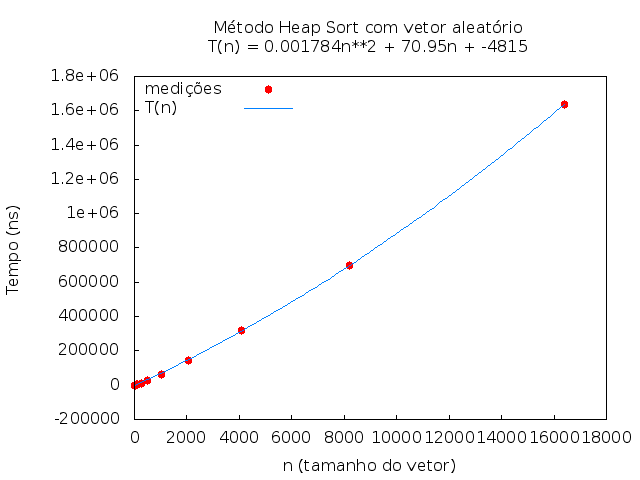
\includegraphics[width=0.7\linewidth]{graficos/HeapSort/vIntAleatorio/vIntAleatorio.png}
  \caption{Parentização Bottom Up - Vetor Decrescente P40}
\end{figure}


\subsection{Vetor Decrescente P50}
Tabela gerada utilizando Parentização Bottom Up com vetores de tamanho n, sendo n = $(2^k)$, de k = 4..14 e inseridos Decrescente P50.
\begin{table}[H]
\centering
\caption{Parentização Bottom Up com vetor Decrescente P50}
\label{my-label}
\begin{tabular}{|l|l|}
\hline
\multicolumn{1}{|c|}{\textbf{Número de Elementos}} & \multicolumn{1}{c|}{\textbf{Tempo de execução em nanosegundos}} \\ \hline
16 & 8230 \\ \hline
32 & 19874 \\ \hline
64 & 138865 \\ \hline
128 & 1119535 \\ \hline
256 & 7674247 \\ \hline
512 & 70240583 \\ \hline
1024 & 1582607779 \\ \hline
\end{tabular}
\end{table}

\begin{figure}[H]
    \centering
    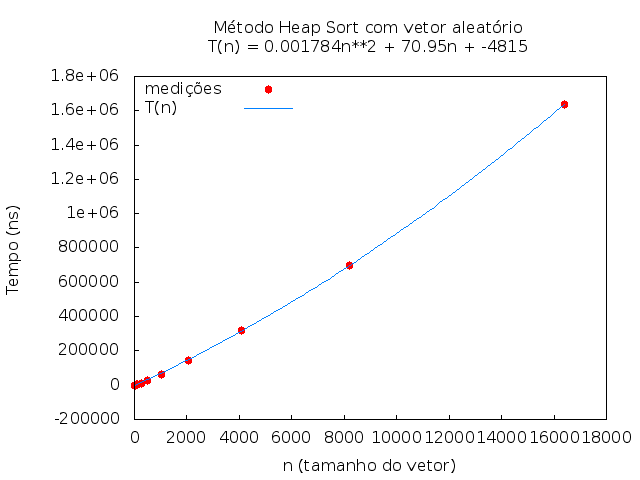
\includegraphics[width=0.7\linewidth]{graficos/HeapSort/vIntAleatorio/vIntAleatorio.png}
  \caption{Parentização Bottom Up - Vetor Decrescente P50}
\end{figure}






\section{Parentização Recursiva}

bLABLABALBALBAL

Tabela gerada utilizando Parentização Recursiva com vetores de tamanho n, sendo n = $(2^k)$, de k = 4..14 e inseridos aleatóriamente, crescente, crescente P10, crescente P20, crescente P30, crescente P40, crescente P50, decrescente, decrescente P10, decrescente P20, decrescente P30, decrescente P40, decrescente P50.
\begin{table}[H]
\centering
\caption{Parentização Recursiva}
\label{my-label}
\begin{tabular}{|l|l|}
\hline
\multicolumn{1}{|c|}{\textbf{Número de Elementos}} & \multicolumn{1}{c|}{\textbf{Tempo de execução em nanosegundos}} \\ \hline
16 & 103633175 \\ \hline
16 & 103633175 \\ \hline
16 & 103633175 \\ \hline
16 & 103633175 \\ \hline
16 & 103633175 \\ \hline
16 & 103633175 \\ \hline
16 & 103633175 \\ \hline
16 & 103633175 \\ \hline
16 & 103633175 \\ \hline
16 & 103633175 \\ \hline
16 & 103633175 \\ \hline
16 & 103633175 \\ \hline
16 & 103633175 \\ \hline
\end{tabular}
\end{table}

\begin{figure}[H]
    \centering
    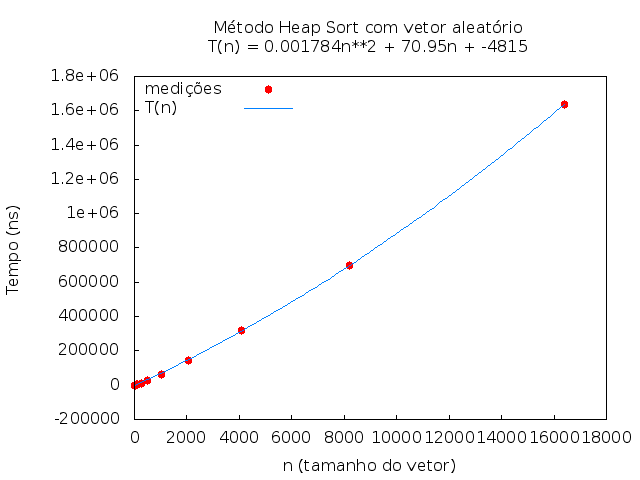
\includegraphics[width=0.7\linewidth]{graficos/HeapSort/vIntAleatorio/vIntAleatorio.png}
  \caption{Parentização Recursiva}
\end{figure}
















\chapter{Estatísticas de Ordem}

Programação dinamica blablabla

\section{Min}

falar um pouco sobre

\subsection{Vetor aleatorio}
Tabela gerada utilizando Min com vetores de tamanho n, sendo n = $(2^k)$, de k = 4..14 e inseridos aleatóriamente.
\begin{table}[H]
\centering
\caption{Min com vetor aleatório}
\label{my-label}
\begin{tabular}{|l|l|}
\hline
\multicolumn{1}{|c|}{\textbf{Número de Elementos}} & \multicolumn{1}{c|}{\textbf{Tempo de execução em nanosegundos}} \\ \hline
16 & 373 \\ \hline
32 & 379 \\ \hline
64 & 417 \\ \hline
128 & 399 \\ \hline
256 & 427 \\ \hline
512 & 477 \\ \hline
1024 & 707 \\ \hline
2048 & 922 \\ \hline
4096 & 1540 \\ \hline
8192 & 3131 \\ \hline
16384 & 7067 \\ \hline
\end{tabular}
\end{table}

\begin{figure}[H]
    \centering
    \includegraphics[width=0.7\linewidth]{graficos/HeapSort/vIntAleatorio/vIntAleatorio.png}
  \caption{Min - Vetor Aleatório}
\end{figure}



\subsection{Vetor Crescente}
Tabela gerada utilizando Min com vetores de tamanho n, sendo n = $(2^k)$, de k = 4..14 e inseridos Crescente.
\begin{table}[H]
\centering
\caption{Min com vetor Crescente}
\label{my-label}
\begin{tabular}{|l|l|}
\hline
\multicolumn{1}{|c|}{\textbf{Número de Elementos}} & \multicolumn{1}{c|}{\textbf{Tempo de execução em nanosegundos}} \\ \hline
16 & 373 \\ \hline
32 & 379 \\ \hline
64 & 417 \\ \hline
128 & 399 \\ \hline
256 & 427 \\ \hline
512 & 477 \\ \hline
1024 & 707 \\ \hline
2048 & 922 \\ \hline
4096 & 1540 \\ \hline
8192 & 3131 \\ \hline
16384 & 7067 \\ \hline
\end{tabular}
\end{table}

\begin{figure}[H]
    \centering
    \includegraphics[width=0.7\linewidth]{graficos/HeapSort/vIntAleatorio/vIntAleatorio.png}
  \caption{Min - Vetor Crescente}
\end{figure}


\subsection{Vetor Crescente P10}
Tabela gerada utilizando Min com vetores de tamanho n, sendo n = $(2^k)$, de k = 4..14 e inseridos Crescente P10.
\begin{table}[H]
\centering
\caption{Min com vetor Crescente P10}
\label{my-label}
\begin{tabular}{|l|l|}
\hline
\multicolumn{1}{|c|}{\textbf{Número de Elementos}} & \multicolumn{1}{c|}{\textbf{Tempo de execução em nanosegundos}} \\ \hline
16 & 373 \\ \hline
32 & 379 \\ \hline
64 & 417 \\ \hline
128 & 399 \\ \hline
256 & 427 \\ \hline
512 & 477 \\ \hline
1024 & 707 \\ \hline
2048 & 922 \\ \hline
4096 & 1540 \\ \hline
8192 & 3131 \\ \hline
16384 & 7067 \\ \hline
\end{tabular}
\end{table}

\begin{figure}[H]
    \centering
    \includegraphics[width=0.7\linewidth]{graficos/HeapSort/vIntAleatorio/vIntAleatorio.png}
  \caption{Min - Vetor Crescente P10}
\end{figure}




\subsection{Vetor Crescente P20}
Tabela gerada utilizando Min com vetores de tamanho n, sendo n = $(2^k)$, de k = 4..14 e inseridos Crescente P20.
\begin{table}[H]
\centering
\caption{Min com vetor Crescente P20}
\label{my-label}
\begin{tabular}{|l|l|}
\hline
\multicolumn{1}{|c|}{\textbf{Número de Elementos}} & \multicolumn{1}{c|}{\textbf{Tempo de execução em nanosegundos}} \\ \hline
16 & 373 \\ \hline
32 & 379 \\ \hline
64 & 417 \\ \hline
128 & 399 \\ \hline
256 & 427 \\ \hline
512 & 477 \\ \hline
1024 & 707 \\ \hline
2048 & 922 \\ \hline
4096 & 1540 \\ \hline
8192 & 3131 \\ \hline
16384 & 7067 \\ \hline
\end{tabular}
\end{table}

\begin{figure}[H]
    \centering
    \includegraphics[width=0.7\linewidth]{graficos/HeapSort/vIntAleatorio/vIntAleatorio.png}
  \caption{Min - Vetor Crescente P20}
\end{figure}





\subsection{Vetor Crescente P30}
Tabela gerada utilizando Min com vetores de tamanho n, sendo n = $(2^k)$, de k = 4..14 e inseridos Crescente P30.
\begin{table}[H]
\centering
\caption{Min com vetor Crescente P30}
\label{my-label}
\begin{tabular}{|l|l|}
\hline
\multicolumn{1}{|c|}{\textbf{Número de Elementos}} & \multicolumn{1}{c|}{\textbf{Tempo de execução em nanosegundos}} \\ \hline
16 & 373 \\ \hline
32 & 379 \\ \hline
64 & 417 \\ \hline
128 & 399 \\ \hline
256 & 427 \\ \hline
512 & 477 \\ \hline
1024 & 707 \\ \hline
2048 & 922 \\ \hline
4096 & 1540 \\ \hline
8192 & 3131 \\ \hline
16384 & 7067 \\ \hline
\end{tabular}
\end{table}

\begin{figure}[H]
    \centering
    \includegraphics[width=0.7\linewidth]{graficos/HeapSort/vIntAleatorio/vIntAleatorio.png}
  \caption{Min - Vetor Crescente P30}
\end{figure}





\subsection{Vetor Crescente P40}
Tabela gerada utilizando Min com vetores de tamanho n, sendo n = $(2^k)$, de k = 4..14 e inseridos Crescente P40.
\begin{table}[H]
\centering
\caption{Min com vetor Crescente P40}
\label{my-label}
\begin{tabular}{|l|l|}
\hline
\multicolumn{1}{|c|}{\textbf{Número de Elementos}} & \multicolumn{1}{c|}{\textbf{Tempo de execução em nanosegundos}} \\ \hline
16 & 373 \\ \hline
32 & 379 \\ \hline
64 & 417 \\ \hline
128 & 399 \\ \hline
256 & 427 \\ \hline
512 & 477 \\ \hline
1024 & 707 \\ \hline
2048 & 922 \\ \hline
4096 & 1540 \\ \hline
8192 & 3131 \\ \hline
16384 & 7067 \\ \hline
\end{tabular}
\end{table}

\begin{figure}[H]
    \centering
    \includegraphics[width=0.7\linewidth]{graficos/HeapSort/vIntAleatorio/vIntAleatorio.png}
  \caption{Min - Vetor Crescente P40}
\end{figure}






\subsection{Vetor Crescente P50}
Tabela gerada utilizando Min com vetores de tamanho n, sendo n = $(2^k)$, de k = 4..14 e inseridos Crescente P50.
\begin{table}[H]
\centering
\caption{Min com vetor Crescente P50}
\label{my-label}
\begin{tabular}{|l|l|}
\hline
\multicolumn{1}{|c|}{\textbf{Número de Elementos}} & \multicolumn{1}{c|}{\textbf{Tempo de execução em nanosegundos}} \\ \hline
16 & 373 \\ \hline
32 & 379 \\ \hline
64 & 417 \\ \hline
128 & 399 \\ \hline
256 & 427 \\ \hline
512 & 477 \\ \hline
1024 & 707 \\ \hline
2048 & 922 \\ \hline
4096 & 1540 \\ \hline
8192 & 3131 \\ \hline
16384 & 7067 \\ \hline
\end{tabular}
\end{table}

\begin{figure}[H]
    \centering
    \includegraphics[width=0.7\linewidth]{graficos/HeapSort/vIntAleatorio/vIntAleatorio.png}
  \caption{Min - Vetor Crescente P50}
\end{figure}




\subsection{Vetor Decrescente}
Tabela gerada utilizando Min com vetores de tamanho n, sendo n = $(2^k)$, de k = 4..14 e inseridos Decrescente.
\begin{table}[H]
\centering
\caption{Min com vetor Decrescente}
\label{my-label}
\begin{tabular}{|l|l|}
\hline
\multicolumn{1}{|c|}{\textbf{Número de Elementos}} & \multicolumn{1}{c|}{\textbf{Tempo de execução em nanosegundos}} \\ \hline
16 & 373 \\ \hline
32 & 379 \\ \hline
64 & 417 \\ \hline
128 & 399 \\ \hline
256 & 427 \\ \hline
512 & 477 \\ \hline
1024 & 707 \\ \hline
2048 & 922 \\ \hline
4096 & 1540 \\ \hline
8192 & 3131 \\ \hline
16384 & 7067 \\ \hline
\end{tabular}
\end{table}

\begin{figure}[H]
    \centering
    \includegraphics[width=0.7\linewidth]{graficos/HeapSort/vIntAleatorio/vIntAleatorio.png}
  \caption{Min - Vetor Decrescente}
\end{figure}




\subsection{Vetor Decrescente P10}
Tabela gerada utilizando Min com vetores de tamanho n, sendo n = $(2^k)$, de k = 4..14 e inseridos Decrescente P10.
\begin{table}[H]
\centering
\caption{Min com vetor Decrescente P10}
\label{my-label}
\begin{tabular}{|l|l|}
\hline
\multicolumn{1}{|c|}{\textbf{Número de Elementos}} & \multicolumn{1}{c|}{\textbf{Tempo de execução em nanosegundos}} \\ \hline
16 & 373 \\ \hline
32 & 379 \\ \hline
64 & 417 \\ \hline
128 & 399 \\ \hline
256 & 427 \\ \hline
512 & 477 \\ \hline
1024 & 707 \\ \hline
2048 & 922 \\ \hline
4096 & 1540 \\ \hline
8192 & 3131 \\ \hline
16384 & 7067 \\ \hline
\end{tabular}
\end{table}

\begin{figure}[H]
    \centering
    \includegraphics[width=0.7\linewidth]{graficos/HeapSort/vIntAleatorio/vIntAleatorio.png}
  \caption{Min - Vetor Decrescente P10}
\end{figure}



\subsection{Vetor Decrescente P20}
Tabela gerada utilizando Min com vetores de tamanho n, sendo n = $(2^k)$, de k = 4..14 e inseridos Decrescente P20.
\begin{table}[H]
\centering
\caption{Min com vetor Decrescente P20}
\label{my-label}
\begin{tabular}{|l|l|}
\hline
\multicolumn{1}{|c|}{\textbf{Número de Elementos}} & \multicolumn{1}{c|}{\textbf{Tempo de execução em nanosegundos}} \\ \hline
16 & 373 \\ \hline
32 & 379 \\ \hline
64 & 417 \\ \hline
128 & 399 \\ \hline
256 & 427 \\ \hline
512 & 477 \\ \hline
1024 & 707 \\ \hline
2048 & 922 \\ \hline
4096 & 1540 \\ \hline
8192 & 3131 \\ \hline
16384 & 7067 \\ \hline
\end{tabular}
\end{table}

\begin{figure}[H]
    \centering
    \includegraphics[width=0.7\linewidth]{graficos/HeapSort/vIntAleatorio/vIntAleatorio.png}
  \caption{Min - Vetor Decrescente P20}
\end{figure}



\subsection{Vetor Decrescente P30}
Tabela gerada utilizando Min com vetores de tamanho n, sendo n = $(2^k)$, de k = 4..14 e inseridos Decrescente P30.
\begin{table}[H]
\centering
\caption{Min com vetor Decrescente P30}
\label{my-label}
\begin{tabular}{|l|l|}
\hline
\multicolumn{1}{|c|}{\textbf{Número de Elementos}} & \multicolumn{1}{c|}{\textbf{Tempo de execução em nanosegundos}} \\ \hline
16 & 373 \\ \hline
32 & 379 \\ \hline
64 & 417 \\ \hline
128 & 399 \\ \hline
256 & 427 \\ \hline
512 & 477 \\ \hline
1024 & 707 \\ \hline
2048 & 922 \\ \hline
4096 & 1540 \\ \hline
8192 & 3131 \\ \hline
16384 & 7067 \\ \hline
\end{tabular}
\end{table}

\begin{figure}[H]
    \centering
    \includegraphics[width=0.7\linewidth]{graficos/HeapSort/vIntAleatorio/vIntAleatorio.png}
  \caption{Min - Vetor Decrescente P30}
\end{figure}




\subsection{Vetor Decrescente P40}
Tabela gerada utilizando Min com vetores de tamanho n, sendo n = $(2^k)$, de k = 4..14 e inseridos Decrescente P40.
\begin{table}[H]
\centering
\caption{Min com vetor Decrescente P40}
\label{my-label}
\begin{tabular}{|l|l|}
\hline
\multicolumn{1}{|c|}{\textbf{Número de Elementos}} & \multicolumn{1}{c|}{\textbf{Tempo de execução em nanosegundos}} \\ \hline
16 & 373 \\ \hline
32 & 379 \\ \hline
64 & 417 \\ \hline
128 & 399 \\ \hline
256 & 427 \\ \hline
512 & 477 \\ \hline
1024 & 707 \\ \hline
2048 & 922 \\ \hline
4096 & 1540 \\ \hline
8192 & 3131 \\ \hline
16384 & 7067 \\ \hline
\end{tabular}
\end{table}

\begin{figure}[H]
    \centering
    \includegraphics[width=0.7\linewidth]{graficos/HeapSort/vIntAleatorio/vIntAleatorio.png}
  \caption{Min - Vetor Decrescente P40}
\end{figure}




\subsection{Vetor Decrescente P50}
Tabela gerada utilizando Min com vetores de tamanho n, sendo n = $(2^k)$, de k = 4..14 e inseridos Decrescente P50.
\begin{table}[H]
\centering
\caption{Min com vetor Decrescente P50}
\label{my-label}
\begin{tabular}{|l|l|}
\hline
\multicolumn{1}{|c|}{\textbf{Número de Elementos}} & \multicolumn{1}{c|}{\textbf{Tempo de execução em nanosegundos}} \\ \hline
16 & 373 \\ \hline
32 & 379 \\ \hline
64 & 417 \\ \hline
128 & 399 \\ \hline
256 & 427 \\ \hline
512 & 477 \\ \hline
1024 & 707 \\ \hline
2048 & 922 \\ \hline
4096 & 1540 \\ \hline
8192 & 3131 \\ \hline
16384 & 7067 \\ \hline
\end{tabular}
\end{table}

\begin{figure}[H]
    \centering
    \includegraphics[width=0.7\linewidth]{graficos/HeapSort/vIntAleatorio/vIntAleatorio.png}
  \caption{Min - Vetor Decrescente P50}
\end{figure}




\section{MinMax}

falar um pouco sobre

\subsection{Vetor aleatorio}
Tabela gerada utilizando MinMax com vetores de tamanho n, sendo n = $(2^k)$, de k = 4..14 e inseridos aleatóriamente.
\begin{table}[H]
\centering
\caption{MinMax com vetor aleatório}
\label{my-label}
\begin{tabular}{|l|l|}
\hline
\multicolumn{1}{|c|}{\textbf{Número de Elementos}} & \multicolumn{1}{c|}{\textbf{Tempo de execução em nanosegundos}} \\ \hline
16 & 628 \\ \hline
32 & 634 \\ \hline
64 & 686 \\ \hline
128 & 492 \\ \hline
256 & 1042 \\ \hline
512 & 806 \\ \hline
1024 & 1087 \\ \hline
2048 & 1250 \\ \hline
4096 & 2139 \\ \hline
8192 & 3898 \\ \hline
16384 & 9144 \\ \hline
\end{tabular}
\end{table}

\begin{figure}[H]
    \centering
    \includegraphics[width=0.7\linewidth]{graficos/HeapSort/vIntAleatorio/vIntAleatorio.png}
  \caption{MinMax - Vetor Aleatório}
\end{figure}




\subsection{Vetor Crescente}
Tabela gerada utilizando MinMax com vetores de tamanho n, sendo n = $(2^k)$, de k = 4..14 e inseridos Crescente.
\begin{table}[H]
\centering
\caption{MinMax com vetor Crescente}
\label{my-label}
\begin{tabular}{|l|l|}
\hline
\multicolumn{1}{|c|}{\textbf{Número de Elementos}} & \multicolumn{1}{c|}{\textbf{Tempo de execução em nanosegundos}} \\ \hline
16 & 628 \\ \hline
32 & 634 \\ \hline
64 & 686 \\ \hline
128 & 492 \\ \hline
256 & 1042 \\ \hline
512 & 806 \\ \hline
1024 & 1087 \\ \hline
2048 & 1250 \\ \hline
4096 & 2139 \\ \hline
8192 & 3898 \\ \hline
16384 & 9144 \\ \hline
\end{tabular}
\end{table}

\begin{figure}[H]
    \centering
    \includegraphics[width=0.7\linewidth]{graficos/HeapSort/vIntAleatorio/vIntAleatorio.png}
  \caption{MinMax - Vetor Crescente}
\end{figure}




\subsection{Vetor Crescente P10}
Tabela gerada utilizando MinMax com vetores de tamanho n, sendo n = $(2^k)$, de k = 4..14 e inseridos Crescente P10.
\begin{table}[H]
\centering
\caption{MinMax com vetor Crescente P10}
\label{my-label}
\begin{tabular}{|l|l|}
\hline
\multicolumn{1}{|c|}{\textbf{Número de Elementos}} & \multicolumn{1}{c|}{\textbf{Tempo de execução em nanosegundos}} \\ \hline
16 & 628 \\ \hline
32 & 634 \\ \hline
64 & 686 \\ \hline
128 & 492 \\ \hline
256 & 1042 \\ \hline
512 & 806 \\ \hline
1024 & 1087 \\ \hline
2048 & 1250 \\ \hline
4096 & 2139 \\ \hline
8192 & 3898 \\ \hline
16384 & 9144 \\ \hline
\end{tabular}
\end{table}

\begin{figure}[H]
    \centering
    \includegraphics[width=0.7\linewidth]{graficos/HeapSort/vIntAleatorio/vIntAleatorio.png}
  \caption{MinMax - Vetor Crescente P10}
\end{figure}





\subsection{Vetor Crescente P20}
Tabela gerada utilizando MinMax com vetores de tamanho n, sendo n = $(2^k)$, de k = 4..14 e inseridos Crescente P20.
\begin{table}[H]
\centering
\caption{MinMax com vetor Crescente P20}
\label{my-label}
\begin{tabular}{|l|l|}
\hline
\multicolumn{1}{|c|}{\textbf{Número de Elementos}} & \multicolumn{1}{c|}{\textbf{Tempo de execução em nanosegundos}} \\ \hline
16 & 628 \\ \hline
32 & 634 \\ \hline
64 & 686 \\ \hline
128 & 492 \\ \hline
256 & 1042 \\ \hline
512 & 806 \\ \hline
1024 & 1087 \\ \hline
2048 & 1250 \\ \hline
4096 & 2139 \\ \hline
8192 & 3898 \\ \hline
16384 & 9144 \\ \hline
\end{tabular}
\end{table}

\begin{figure}[H]
    \centering
    \includegraphics[width=0.7\linewidth]{graficos/HeapSort/vIntAleatorio/vIntAleatorio.png}
  \caption{MinMax - Vetor Crescente P20}
\end{figure}




\subsection{Vetor Crescente P30}
Tabela gerada utilizando MinMax com vetores de tamanho n, sendo n = $(2^k)$, de k = 4..14 e inseridos Crescente P30.
\begin{table}[H]
\centering
\caption{MinMax com vetor Crescente P30}
\label{my-label}
\begin{tabular}{|l|l|}
\hline
\multicolumn{1}{|c|}{\textbf{Número de Elementos}} & \multicolumn{1}{c|}{\textbf{Tempo de execução em nanosegundos}} \\ \hline
16 & 628 \\ \hline
32 & 634 \\ \hline
64 & 686 \\ \hline
128 & 492 \\ \hline
256 & 1042 \\ \hline
512 & 806 \\ \hline
1024 & 1087 \\ \hline
2048 & 1250 \\ \hline
4096 & 2139 \\ \hline
8192 & 3898 \\ \hline
16384 & 9144 \\ \hline
\end{tabular}
\end{table}

\begin{figure}[H]
    \centering
    \includegraphics[width=0.7\linewidth]{graficos/HeapSort/vIntAleatorio/vIntAleatorio.png}
  \caption{MinMax - Vetor Crescente P30}
\end{figure}





\subsection{Vetor Crescente P40}
Tabela gerada utilizando MinMax com vetores de tamanho n, sendo n = $(2^k)$, de k = 4..14 e inseridos Crescente P40.
\begin{table}[H]
\centering
\caption{MinMax com vetor Crescente P40}
\label{my-label}
\begin{tabular}{|l|l|}
\hline
\multicolumn{1}{|c|}{\textbf{Número de Elementos}} & \multicolumn{1}{c|}{\textbf{Tempo de execução em nanosegundos}} \\ \hline
16 & 628 \\ \hline
32 & 634 \\ \hline
64 & 686 \\ \hline
128 & 492 \\ \hline
256 & 1042 \\ \hline
512 & 806 \\ \hline
1024 & 1087 \\ \hline
2048 & 1250 \\ \hline
4096 & 2139 \\ \hline
8192 & 3898 \\ \hline
16384 & 9144 \\ \hline
\end{tabular}
\end{table}

\begin{figure}[H]
    \centering
    \includegraphics[width=0.7\linewidth]{graficos/HeapSort/vIntAleatorio/vIntAleatorio.png}
  \caption{MinMax - Vetor Crescente P40}
\end{figure}




\subsection{Vetor Crescente P50}
Tabela gerada utilizando MinMax com vetores de tamanho n, sendo n = $(2^k)$, de k = 4..14 e inseridos Crescente P50.
\begin{table}[H]
\centering
\caption{MinMax com vetor Crescente P50}
\label{my-label}
\begin{tabular}{|l|l|}
\hline
\multicolumn{1}{|c|}{\textbf{Número de Elementos}} & \multicolumn{1}{c|}{\textbf{Tempo de execução em nanosegundos}} \\ \hline
16 & 628 \\ \hline
32 & 634 \\ \hline
64 & 686 \\ \hline
128 & 492 \\ \hline
256 & 1042 \\ \hline
512 & 806 \\ \hline
1024 & 1087 \\ \hline
2048 & 1250 \\ \hline
4096 & 2139 \\ \hline
8192 & 3898 \\ \hline
16384 & 9144 \\ \hline
\end{tabular}
\end{table}

\begin{figure}[H]
    \centering
    \includegraphics[width=0.7\linewidth]{graficos/HeapSort/vIntAleatorio/vIntAleatorio.png}
  \caption{MinMax - Vetor Crescente P50}
\end{figure}





\subsection{Vetor Decrescente}
Tabela gerada utilizando MinMax com vetores de tamanho n, sendo n = $(2^k)$, de k = 4..14 e inseridos Decrescente.
\begin{table}[H]
\centering
\caption{MinMax com vetor Decrescente}
\label{my-label}
\begin{tabular}{|l|l|}
\hline
\multicolumn{1}{|c|}{\textbf{Número de Elementos}} & \multicolumn{1}{c|}{\textbf{Tempo de execução em nanosegundos}} \\ \hline
16 & 628 \\ \hline
32 & 634 \\ \hline
64 & 686 \\ \hline
128 & 492 \\ \hline
256 & 1042 \\ \hline
512 & 806 \\ \hline
1024 & 1087 \\ \hline
2048 & 1250 \\ \hline
4096 & 2139 \\ \hline
8192 & 3898 \\ \hline
16384 & 9144 \\ \hline
\end{tabular}
\end{table}

\begin{figure}[H]
    \centering
    \includegraphics[width=0.7\linewidth]{graficos/HeapSort/vIntAleatorio/vIntAleatorio.png}
  \caption{MinMax - Vetor Decrescente}
\end{figure}



\subsection{Vetor Decrescente P10}
Tabela gerada utilizando MinMax com vetores de tamanho n, sendo n = $(2^k)$, de k = 4..14 e inseridos Decrescente P10.
\begin{table}[H]
\centering
\caption{MinMax com vetor Decrescente P10}
\label{my-label}
\begin{tabular}{|l|l|}
\hline
\multicolumn{1}{|c|}{\textbf{Número de Elementos}} & \multicolumn{1}{c|}{\textbf{Tempo de execução em nanosegundos}} \\ \hline
16 & 628 \\ \hline
32 & 634 \\ \hline
64 & 686 \\ \hline
128 & 492 \\ \hline
256 & 1042 \\ \hline
512 & 806 \\ \hline
1024 & 1087 \\ \hline
2048 & 1250 \\ \hline
4096 & 2139 \\ \hline
8192 & 3898 \\ \hline
16384 & 9144 \\ \hline
\end{tabular}
\end{table}

\begin{figure}[H]
    \centering
    \includegraphics[width=0.7\linewidth]{graficos/HeapSort/vIntAleatorio/vIntAleatorio.png}
  \caption{MinMax - Vetor Decrescente P10}
\end{figure}




\subsection{Vetor Decrescente P20}
Tabela gerada utilizando MinMax com vetores de tamanho n, sendo n = $(2^k)$, de k = 4..14 e inseridos Decrescente P20.
\begin{table}[H]
\centering
\caption{MinMax com vetor Decrescente P20}
\label{my-label}
\begin{tabular}{|l|l|}
\hline
\multicolumn{1}{|c|}{\textbf{Número de Elementos}} & \multicolumn{1}{c|}{\textbf{Tempo de execução em nanosegundos}} \\ \hline
16 & 628 \\ \hline
32 & 634 \\ \hline
64 & 686 \\ \hline
128 & 492 \\ \hline
256 & 1042 \\ \hline
512 & 806 \\ \hline
1024 & 1087 \\ \hline
2048 & 1250 \\ \hline
4096 & 2139 \\ \hline
8192 & 3898 \\ \hline
16384 & 9144 \\ \hline
\end{tabular}
\end{table}

\begin{figure}[H]
    \centering
    \includegraphics[width=0.7\linewidth]{graficos/HeapSort/vIntAleatorio/vIntAleatorio.png}
  \caption{MinMax - Vetor Decrescente P20}
\end{figure}



\subsection{Vetor Decrescente P30}
Tabela gerada utilizando MinMax com vetores de tamanho n, sendo n = $(2^k)$, de k = 4..14 e inseridos Decrescente P30.
\begin{table}[H]
\centering
\caption{MinMax com vetor Decrescente P30}
\label{my-label}
\begin{tabular}{|l|l|}
\hline
\multicolumn{1}{|c|}{\textbf{Número de Elementos}} & \multicolumn{1}{c|}{\textbf{Tempo de execução em nanosegundos}} \\ \hline
16 & 628 \\ \hline
32 & 634 \\ \hline
64 & 686 \\ \hline
128 & 492 \\ \hline
256 & 1042 \\ \hline
512 & 806 \\ \hline
1024 & 1087 \\ \hline
2048 & 1250 \\ \hline
4096 & 2139 \\ \hline
8192 & 3898 \\ \hline
16384 & 9144 \\ \hline
\end{tabular}
\end{table}

\begin{figure}[H]
    \centering
    \includegraphics[width=0.7\linewidth]{graficos/HeapSort/vIntAleatorio/vIntAleatorio.png}
  \caption{MinMax - Vetor Decrescente P30}
\end{figure}





\subsection{Vetor Decrescente P40}
Tabela gerada utilizando MinMax com vetores de tamanho n, sendo n = $(2^k)$, de k = 4..14 e inseridos Decrescente P40.
\begin{table}[H]
\centering
\caption{MinMax com vetor Decrescente P40}
\label{my-label}
\begin{tabular}{|l|l|}
\hline
\multicolumn{1}{|c|}{\textbf{Número de Elementos}} & \multicolumn{1}{c|}{\textbf{Tempo de execução em nanosegundos}} \\ \hline
16 & 628 \\ \hline
32 & 634 \\ \hline
64 & 686 \\ \hline
128 & 492 \\ \hline
256 & 1042 \\ \hline
512 & 806 \\ \hline
1024 & 1087 \\ \hline
2048 & 1250 \\ \hline
4096 & 2139 \\ \hline
8192 & 3898 \\ \hline
16384 & 9144 \\ \hline
\end{tabular}
\end{table}

\begin{figure}[H]
    \centering
    \includegraphics[width=0.7\linewidth]{graficos/HeapSort/vIntAleatorio/vIntAleatorio.png}
  \caption{MinMax - Vetor Decrescente P40}
\end{figure}





\subsection{Vetor Decrescente P50}
Tabela gerada utilizando MinMax com vetores de tamanho n, sendo n = $(2^k)$, de k = 4..14 e inseridos Decrescente P50.
\begin{table}[H]
\centering
\caption{MinMax com vetor Decrescente P50}
\label{my-label}
\begin{tabular}{|l|l|}
\hline
\multicolumn{1}{|c|}{\textbf{Número de Elementos}} & \multicolumn{1}{c|}{\textbf{Tempo de execução em nanosegundos}} \\ \hline
16 & 628 \\ \hline
32 & 634 \\ \hline
64 & 686 \\ \hline
128 & 492 \\ \hline
256 & 1042 \\ \hline
512 & 806 \\ \hline
1024 & 1087 \\ \hline
2048 & 1250 \\ \hline
4096 & 2139 \\ \hline
8192 & 3898 \\ \hline
16384 & 9144 \\ \hline
\end{tabular}
\end{table}

\begin{figure}[H]
    \centering
    \includegraphics[width=0.7\linewidth]{graficos/HeapSort/vIntAleatorio/vIntAleatorio.png}
  \caption{MinMax - Vetor Decrescente P50}
\end{figure}


%para ajuda
%\lstinputlisting[label={arq:prog1.c}, language=C, caption={Módulo Mínimo C}]{codigos/MiniC/prog1.c}
%\lstinputlisting[label={arq:prog4.c}, language=C, caption={Atribuição de uma soma de inteiros a uma variável C}]{codigos/MiniC/prog4.c}
%\begin{terminal}
%> sudo apt-get install llvm
%> sudo apt-get install clang
%\end{terminal}

\chapter{Referências}
\href{https://pt.wikipedia.org/wiki/Insertion_sort}{Insertion Sort}\\
\href{https://pt.wikipedia.org/wiki/Merge_sort}{Merge Sort}\\
\href{https://pt.wikipedia.org/wiki/Heapsort}{Heap Sort}\\
\href{https://en.wikipedia.org/wiki/Quicksort}{Quick Sort}\\
\href{https://pt.wikipedia.org/wiki/Counting_sort}{Counting Sort}\\
\href{https://en.wikipedia.org/wiki/Radix_sort}{Radix Sort}\\
\href{https://en.wikipedia.org/wiki/Bucket_sort}{Bucket Sort}\\
Introduction to algorithms 3rd Edition,Cormen, Thomas H,2009
  
\end{document} 
